\documentclass{report}
\usepackage{textcomp,amsmath,appendix}
\usepackage{graphicx}
%\usepackage{makeidx}
\usepackage[colorlinks=true]{hyperref}
\usepackage{tex4ht}
%\usepackage[style=authoryear,backend=biber]{biblatex}


\title{Addendum : Project 4C \\Integrated Analysis of Room Performance}
\author{Michael Novak} %, Shaun Brandt, Mandar Patil, Hema Kumar, and Yu Yang}


\begin{document}

\maketitle
%\pagestyle{empty}




\begin{abstract}
Using postmortem datasets collected at the PNNL's Energy Smart Data Center (ESDC) facility, an integrated analysis of room performance is conducted. 
Overall room performance, concerning power and cooling, is best captured by chiller metrics.
Temporal data-mining techniques are used in an effort to possibly characterize sustainability measures of the patterns mined from these metrics. 


%An analysis suite, written in Haskell and {\tt Gnuplot},
%is used to produce a novel visualization of clustering overlays on the time-series data for five chiller metrics, in an attempt to discover `motifs'.

 \end{abstract}



\chapter*{Introduction}
%\doublespacing

 %\section{Data Visualization}
 %An analysis suite, written in Haskell and {\tt Gnuplot}, has been created to
 %produces quantitative visualizations of various cooling related metrics concerning the given {\tt RAWDATA}, described below. It uses temporal data-mining technique to produce a novel visualization of cluster overlays on the time-series data for five chiller metrics, in an attempt to discover `motifs' (inspired by work found in \cite{Patnaik2009}).

\section*{Data}
We are using two postmortem datasets collected at the PNNL's ESDC:
\verb=LD_A1_56p_2ppn_28n_IO-BASIC_even_RAWDATA= (LD) and \verb=HD_A1_224p_8ppn_28n_RAWDATA= (HD).
This data seems to correspond to the experiments in \cite{Karavanic2011}: 

  %\item Postmortem data gotten from \verb=/u/karavan/Public= at \verb=rita.cat.pdx 
  \begin{itemize}

 \item The LD dataset---Low-Density Even-Distribution Workload---was collected by FRED \date{2011-05-05}.
  \item The HD dataset---High-Density Workload---was collected by FRED \date{2011-04-25}.
  \item  \begin{quote}
      All of the power and cooling data measured by FRED [Fundamental Research in Energy efficient Data centers, an analysis software tool developed at PNNL] sensors is collected into a central FRED database, using an independent data network.    
    \end{quote}

  \item The workloads consist of MPI tasks split into three trials t01--03.
  \item   
    \begin{quote}
      In the HD schedules, the 224 processes ran on 28 nodes (eight processes per node) all housed in a single rack.
    \end{quote}
\item
   \begin{quote}
     The nodes are connected via a DDR InfiniBand 1-layer fat tree; one rack (A2) contains the networking equipment and seven racks (A1, A3--4, B1--4) are for the compute nodes.
   \end{quote}

 \item
\begin{quote}
In the low density LD schedules, the 224 processes executed on 112 nodes, with two processes per node, and the processes were spread across racks B1, B2, B3, and B4.
 \end{quote}  
 \item
 \begin{quote}
Low Density Even Distribution -- In this set, we used
racks B1, B2, B3, and B4; and we scheduled two MPI
tasks per node, using all of the nodes in all four racks.
 \end{quote}

     \end{itemize}


 \subsection*{Power \& Cooling}

 Power consumption is a likely concern for the ESDC; though only 7.63\textcent{} per kWh, in Oregon. Tables \ref{t1} and \ref{t2} include the average power consumption of each rack over the LD and HD trials according to the postmortem data. % It was hard to tell whether the gradient of one line was steeper than another, in the LD set; hence the accompanying tables were created to show overall kWh increase per trial, and to further scrutinize power consumption within the racks. 


A sure concern for the ESDC is overheating.
Air cooling attempts to dissipate some of the heat generated by the CPUs. A useful metric for estimating cooling effort is the Node Air Delta.
Tables \ref{t1} and \ref{t2} include the average CPU temperatures and Node Air Delta of each rack over the LD and HD trials. Unfortunately, the postmortem data is badly corrupted by faulty sensor readings.
Negative, and ludicrously high, temperature values had to be filtered from the true readings. For CPU temperature, the filtering range was $72<temp<150$.
For Node Air Delta, the filtering range was $0<\Delta temp<40$.

\begin{table}[!h]
  \centering
   \centerline{Total kWh increase.}
   \begin{tabular}{r|ccccccc}\cline{2-8}
\tt PowerUnit PowerKWH&$\bf A1$&$\bf A3$&$\bf A4$&$\bf B1$&$\bf B2$&$\bf B3$&$\bf B4$\\\hline
\bf t01& 1.28& 1.03& 1.07& 1.11& 1.17& 1.31& 1.27\\
\bf t02& 1.28& 1.03& 1.06& 1.11& 1.17& 1.31& 1.27\\
\bf t03& 1.30& 1.05& 1.09& 1.13& 1.19& 1.33& 1.35\\
\hline
\tt Total PowerUnit& 1& 1& 1& 1& 1& 1& 1\\
\end{tabular}
\\
   \vspace{1cm}
   \centerline{Average Per-Node, Per-CPU, CPU Temperature Average for Each Rack (within $72<{\tt Temp}<150$)}
   \begin{tabular}{r|ccccccc}\cline{2-8}
\tt CPU Temp&$\bf A1$&$\bf A3$&$\bf A4$&$\bf B1$&$\bf B2$&$\bf B3$&$\bf B4$\\\hline
\bf t01& 97.18& 83.52& 81.71& 100.15& 89.51& 94.54& 110.43\\
\bf t02& 104.83& 83.99& 82.30& 100.44& 89.75& 94.22& 111.05\\
\bf t03& 116.73& 83.89& 82.26& 100.42& 89.68& 97.33& 111.66\\
\hline
\tt Total CPU& 37& 41& 4& 5& 6& 4& 5\\
\end{tabular}
\\
   \vspace{1cm}
   \centerline{Maximum Per-Node, Per-CPU, CPU Temperature Maximum for Each Rack (within $72<{\tt Temp}<150$)}
   \begin{tabular}{r|ccccccc}\cline{2-8}
\tt CPU Temp&$\bf A1$&$\bf A3$&$\bf A4$&$\bf B1$&$\bf B2$&$\bf B3$&$\bf B4$\\\hline
\bf t01& 107.68& 141.97& 85.05& 127.94& 91.73& 106.14& 120.02\\
\bf t02& 126.13& 142.13& 85.20& 127.94& 91.86& 106.93& 120.95\\
\bf t03& 126.13& 142.13& 85.20& 127.76& 91.86& 108.96& 120.95\\
\hline
\tt Total CPU& 37& 41& 4& 5& 6& 4& 5\\
\end{tabular}
\\
   \vspace{1cm}
   \centerline{Average Per-Node Air Temperature Delta for Each Rack (within $0<\Delta{\tt Temp}<40$)}
   \begin{tabular}{r|ccccccc}\cline{2-8}
\tt NodeAir Delta&$\bf A1$&$\bf A3$&$\bf A4$&$\bf B1$&$\bf B2$&$\bf B3$&$\bf B4$\\\hline
\bf t01& 26.80& 26.20& 26.62& 24.52& 25.28& 24.37& 26.24\\
\bf t02& 27.43& 26.06& 26.44& 24.76& 25.28& 24.43& 26.92\\
\bf t03& 29.16& 25.87& 26.66& 24.16& 25.30& 24.38& 27.17\\
\hline
\tt Total NodeAir& 23& 23& 21& 25& 23& 23& 15\\
\end{tabular}
\\
   \caption{{\bf Low-Density Workload.} To filter out faulty sensor readings, the component temperatures counted do not include every node in every rack; see the counts below each table.\label{t1}}
\end{table}

%%%%%%%%%%%%%%%%%%%%%%%%%%%%%%%%%%%%%%%%%%%%%%%%%%%%%%%%%%%%%%%%%%%%%%%%%%%%%%%
\begin{table}[!h]
  \centering
   \centerline{Total kWh increase.}
   \begin{tabular}{r|ccccccc}\cline{2-8}
\tt PowerUnit PowerKWH&$\bf A1$&$\bf A3$&$\bf A4$&$\bf B1$&$\bf B2$&$\bf B3$&$\bf B4$\\\hline
\bf t01& 1.28& 1.03& 1.07& 1.11& 1.17& 1.31& 1.27\\
\bf t02& 1.28& 1.03& 1.06& 1.11& 1.17& 1.31& 1.27\\
\bf t03& 1.30& 1.05& 1.09& 1.13& 1.19& 1.33& 1.35\\
\hline
\tt Total PowerUnit& 1& 1& 1& 1& 1& 1& 1\\
\end{tabular}
\\
   \vspace{1cm}
   \centerline{Average Per-Node, Per-CPU, CPU Temperature Average for Each Rack (within $72<{\tt Temp}<150$)}
   \begin{tabular}{r|ccccccc}\cline{2-8}
\tt CPU Temp&$\bf A1$&$\bf A3$&$\bf A4$&$\bf B1$&$\bf B2$&$\bf B3$&$\bf B4$\\\hline
\bf t01& 97.18& 83.52& 81.71& 100.15& 89.51& 94.54& 110.43\\
\bf t02& 104.83& 83.99& 82.30& 100.44& 89.75& 94.22& 111.05\\
\bf t03& 116.73& 83.89& 82.26& 100.42& 89.68& 97.33& 111.66\\
\hline
\tt Total CPU& 37& 41& 4& 5& 6& 4& 5\\
\end{tabular}
\\
   \vspace{1cm}
   \centerline{Maximum Per-Node, Per-CPU, CPU Temperature Maximum for Each Rack (within $72<{\tt Temp}<150$)}
   \begin{tabular}{r|ccccccc}\cline{2-8}
\tt CPU Temp&$\bf A1$&$\bf A3$&$\bf A4$&$\bf B1$&$\bf B2$&$\bf B3$&$\bf B4$\\\hline
\bf t01& 107.68& 141.97& 85.05& 127.94& 91.73& 106.14& 120.02\\
\bf t02& 126.13& 142.13& 85.20& 127.94& 91.86& 106.93& 120.95\\
\bf t03& 126.13& 142.13& 85.20& 127.76& 91.86& 108.96& 120.95\\
\hline
\tt Total CPU& 37& 41& 4& 5& 6& 4& 5\\
\end{tabular}
\\
   \vspace{1cm}
   \centerline{Average Per-Node Air Temperature Delta for Each Rack (within $0<\Delta{\tt Temp}<40$)}
   \begin{tabular}{r|ccccccc}\cline{2-8}
\tt NodeAir Delta&$\bf A1$&$\bf A3$&$\bf A4$&$\bf B1$&$\bf B2$&$\bf B3$&$\bf B4$\\\hline
\bf t01& 26.80& 26.20& 26.62& 24.52& 25.28& 24.37& 26.24\\
\bf t02& 27.43& 26.06& 26.44& 24.76& 25.28& 24.43& 26.92\\
\bf t03& 29.16& 25.87& 26.66& 24.16& 25.30& 24.38& 27.17\\
\hline
\tt Total NodeAir& 23& 23& 21& 25& 23& 23& 15\\
\end{tabular}
\\
   \caption{{\bf High-Density Workload.} To filter out faulty sensor readings, the component temperatures counted do not include every node in every rack; see the counts below each table.\label{t2}}


\end{table}



The racks equipped with TMUs provide additional cooling infrastructure.
The degree of cooling which the TMU provides is captured by the water-temperature-delta metric. Another useful metric is the manifold pressure---the mass flow rate of hot/cold water.
Only the LD dataset had useful TMU readings.

%Evidently, trial 3 (t03) involved slightly more energy intensive application processes.

%Are we ever going to get PerfTrack and have the data organized in PostgreSQL?
%perhaps it will be easy to gather the data necessary to make a chart like the one depicted on page 440 of \url{http://web.cecs.pdx.edu/~karavan/csg533/karavanic_PDCS2011.pdf}.
% Chiller utilization measurements were collected by FRED at 30 second intervals; so, for simplicity, each trial's time series starts at 0 and is incremented accordingly.
Overall room performance, concerning power and cooling, is best captured by chiller metrics.
 \subsection*{Chillers}

Within the cooling infrastructure, most of the energy is spent on chillers, which refrigerate the water used to extract heat from the equipment in the data center.
 Chillers keep data centers from overheating and hence keep them properly functioning.
 %Chiller metrics capture the overall performance of the data center's cooling infrastructure.
 While one unit may be sufficient for a small data center, several units operating as an ensemble are required to satisfy the cooling demand of a large data center.

  The ESDC is equipped with 5 chillers units. 
 Three chiller units ($C_1,C_2,C_4$) were used for the LD trials, and only two ($C_1,C_4$) were used for the HD trials---as evidenced by KW consumption. 
The following chiller metrics, derived from \cite{Patnaik2011}, were extracted from the LD and HD datasets.
 \begin{itemize}
   \item
   {\bf Data-center cooling load.} This is the amount of heat that is generated (and thus needs to be dissipated) at a data center. It is approximately equivalent to the power consumed by the equipment since almost all of it is dissipated as heat. It is commonly specified in kilowatts (KW).
 \item
   {\bf COP.} The coefficient of performance (COP) of a chiller unit indicates how efficiently the unit provides cooling, and, is defined as the ratio between the cooling provided and the power consumed, i.e.,
   \begin{equation*}
     COP_i = \frac{L_i}{P_i}\label{cop}
 \end{equation*}
where $L_i$ is the cooling load on the $i$th chiller unit and $P_i$ is the power consumed by it.
\item {\bf Chiller utilization.} Chiller utilization depends on the degree of cooling provided; i.e., the difference between the inlet and outlet water temperatures ({\tt CHILLER WATER-TEMP DELTA} and {\tt CONDENSER WATER-TEMP DELTA}).
\end{itemize}

When these chiller metrics are plotted, oscillations can be observed.
     High amplitude and frequent variations in utilization due to varying load or some failure condition result in decreased lifespan, and, thus, need to be minimized.
 Although operating curves for individual chiller units exist, no model is available for operation of an ensemble, especially one consisting of heterogeneous units.



 \section*{Data Mining}
\newtheorem{mydef}{Definition}


\begin{mydef} 
   A multivariate time series $T = \langle t_1,\dots, t_m\rangle$ is an ordered set of real-valued vectors of a particular variable. Each real-valued vector $t_i$ captures the utilizations across all the chiller units.
 \end{mydef}

     \begin{quote}
Motifs are repetitive patterns of occurrence in time-series data. In understanding multivariate time-series data about chiller utilizations, we seek to identify motifs that underly how different chillers are involved in meeting the varying demand posed by data centers. We would like to identify regions of time-series progression that demonstrate better/improved sustainability measures than others
   \cite[p. \;34:7]{Patnaik2011}.\end{quote}


 \subsection*{Approach}
% Gaussian clusters discovered by EM clustering with $k=3$, over the three trials for the Chiller metrics, produced the best results.  
First, chiller metrics are extracted from the datasets by scripting into their file systems and manipulating the data as vectors with Haskell.
For clustering, ELKI (release 0.4.1 \cite{Achtert}) is used. The algorithms being used are: $k$-means and expectation maximum (EM). 
A Haskell script formats metric data and feeds it to ELKI.
The input data is labeled in such a way that the time-series information can be retrieved after clustering; hence making it possible for cluster transitions to be overlaid on the time series across each of the three trials.
ELKI produces clustering files. Then a Haskell script reads all the cluster files and stores the data points in a Map according to their cluster labels {\tt (trial, SEC)}. Next, {\tt Gnuplot} dat files are created for each trial by looking up data points in the Map and sorting them by time.
The cluster transitions can be seen by overlaying the time series with shades of color representing clusters. 
{\tt Gnuplot} scripts are generated to do this shading. Finally, the Haskell script executes {\tt Gnuplot} on all the {\tt Gnuplot} scripts, which are rendered as PNG images.

This gives an intuitive feel for how a learning algorithm could be built to detect motifs:
You look at the time series to detect motifs, then see if they are captured by transitions of cluster shadings.
These transitions can be used to encode the multivariate numeric data into symbolic form, which can serve as the input to frequent episode mining.
The color shadings make it easy for a human to see what possible motifs the AI would choose using various clustering parameters, hence the human can guide the AI to use the best clustering parameters. 
Colors had to be chosen carefully to be distinguishable and not clash with the plots. The color schemes used were derived from \url{http://www.sron.nl/~pault/colourschemes.pdf}.


\begin{itemize}
  \item Code $\to$ \url{https://github.com/mmlxiv/Data-Analysis_Group4c}
\end{itemize}
%Note: TMU metrics could be analysed in the same way as chiller metrics; but, this was left undone because 
%the HD dataset did not contain usefull TMU metrics.
%It is kind of futile trying to find motifs in the LD dataset, at such a fine granularity with such short lived trials.
% Naively thinking the three trials for each workload (LD \& HD) could be clustered on their chiller metrics led to the automated analysis captured in the cluster-overlayed time-series figures in Appendix D \& F.




 \section*{Reflections \& Future}
This project was a first step toward developing algorithms for processing multivariate time-series data to characterize sustainability measures of the patterns mined.
\begin{itemize}
  \item TMU metrics could be analysed in the same way as chiller metrics; this was left undone because 
the HD dataset did not contain useful TMU metrics.
%\item It is kind of futile trying to find motifs in the LD dataset, at such a fine granularity with such short lived trials.
   \item It would be nice if FRED measurements were stored in a NoSQL graph database. Having the data structured as a graph seems like it would make the data easier to navigate. 
   \item Mining FRED sensor streams, directly, could give a real-time perspective into ESDC behavior so that strategies could be identified to improve efficiency metrics.
\item  Meaningful analysis might be carried out with a more extensive amount of ESDC data.
Example: \cite[pp. \;34:14--34:16 (see Tables I--V)]{Patnaik2011}

  %  \item The temporal data-mining technique of overlaying clusters on the time series, described in \cite{Patnaik2009,Patnaik2011}, was tested on Chiller data. Though, it was difficult to find motifs at such a fine granularity, with our limited data.
  
\item An advanced machine learning infrastructure could be built using Dynamic Bayesian Networks to infer diagnostic predictions (e.g. the CAMAS framework in \cite[p. \;34:8 (see Fig 5.)]{Patnaik2011}).
\end{itemize}


     % \item It would be nice if we could get at the FRED measurements through a cloud-based data store---perhaps a graph database.  
  
 

%%%%%%%%%%%%%%%%%%%%%%%%%%%%%%%%%%%%%%%%%%%%%%%%%%%%%%%%%%%%%%%%%%%%%%%%%%%%%%%





%\nocite{*}
\bibliographystyle{plain}
\bibliography{index}

\tableofcontents

\appendix

\part{Low-Density Workload Visualizations}
\chapter{Metrics : Power Unit, Thermal Management Unit (TMU), and Chiller}
\begin{figure}[!h]
\centerline{\bfseries\large Low-Density Workload : Trials 1--3}\\
\fbox{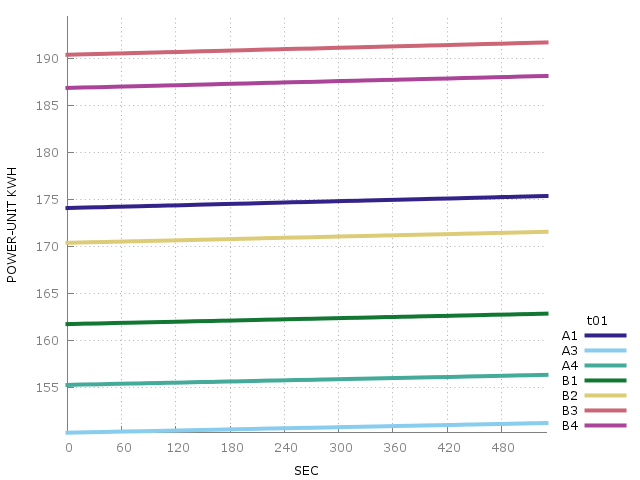
\includegraphics[bb=0 0 640 480, width=5in]{gnu/ld/plot/PowerKWH_t01.png}}
\fbox{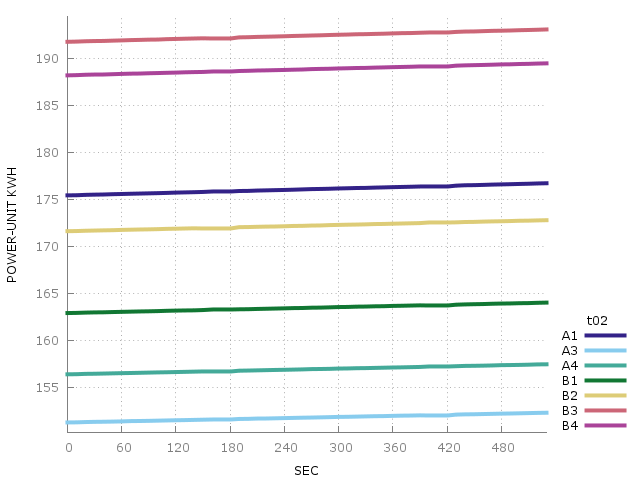
\includegraphics[bb=0 0 640 480, width=5in]{gnu/ld/plot/PowerKWH_t02.png}}
\fbox{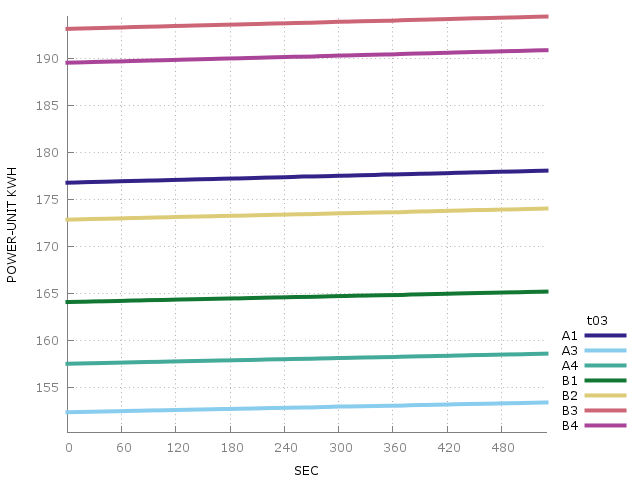
\includegraphics[bb=0 0 640 480, width=5in]{gnu/ld/plot/PowerKWH_t03.png}}
\caption{Racks A1, A3, A4, B1--4; Power-unit kWh increase (7.63\textcent{} per kWh, in Oregon).}
\end{figure}
\begin{figure}[!h]
\centerline{\bfseries\large Low-Density Workload : Trials 1--3}\\
\fbox{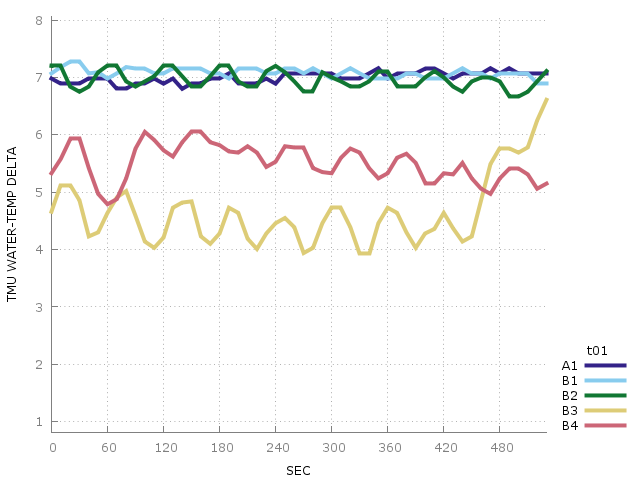
\includegraphics[bb=0 0 640 480, width=5in]{gnu/ld/plot/TMU_WTD_t01.png}}
\fbox{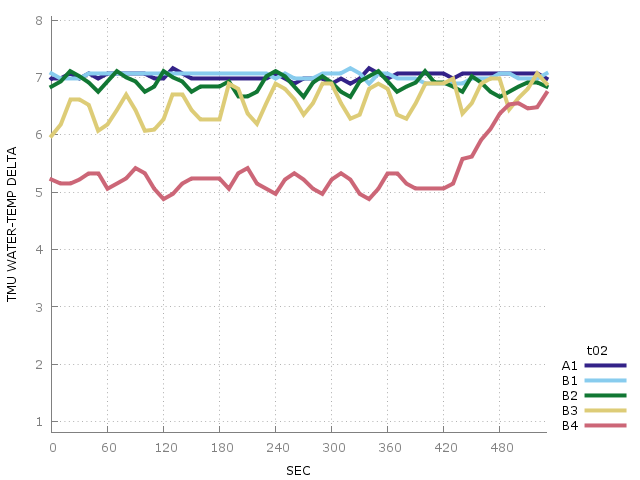
\includegraphics[bb=0 0 640 480, width=5in]{gnu/ld/plot/TMU_WTD_t02.png}}
\fbox{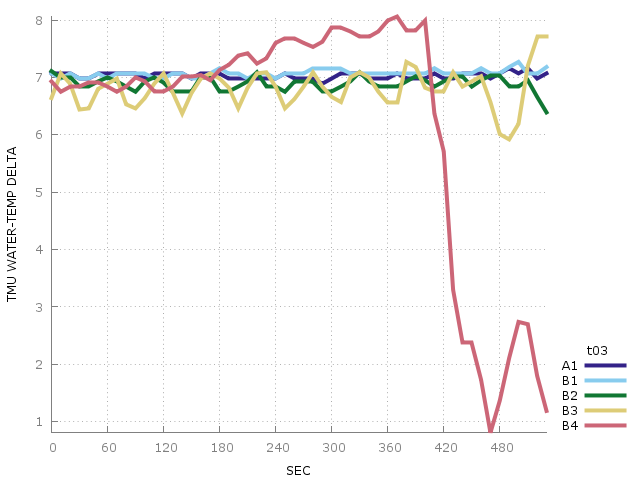
\includegraphics[bb=0 0 640 480, width=5in]{gnu/ld/plot/TMU_WTD_t03.png}}
\caption{Racks A1, B1--4; TMU water-temperature delta, which is obtained by subtracting inlet from outlet temperatures.}
\end{figure}
\begin{figure}[!h]
\centerline{\bfseries\large Low-Density Workload : Trials 1--3}\\
\fbox{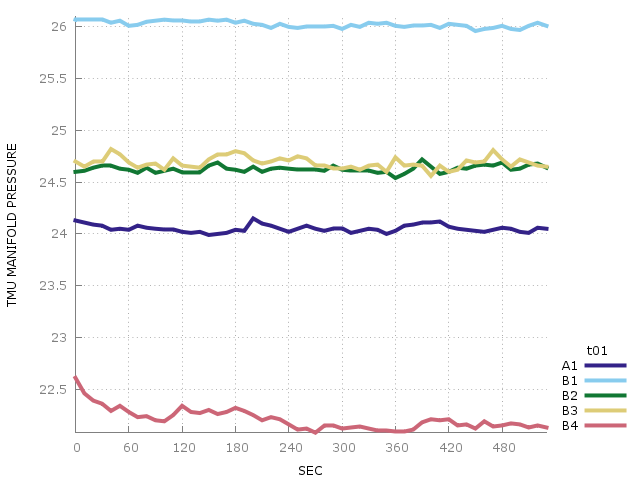
\includegraphics[bb=0 0 640 480, width=5in]{gnu/ld/plot/ManifoldPress_t01.png}}
\fbox{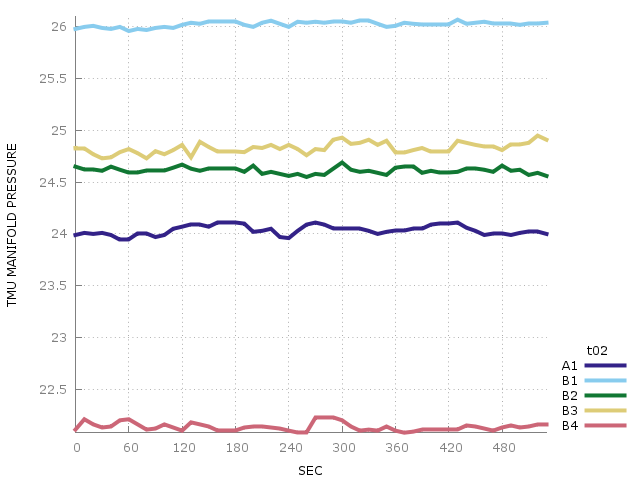
\includegraphics[bb=0 0 640 480, width=5in]{gnu/ld/plot/ManifoldPress_t02.png}}
\fbox{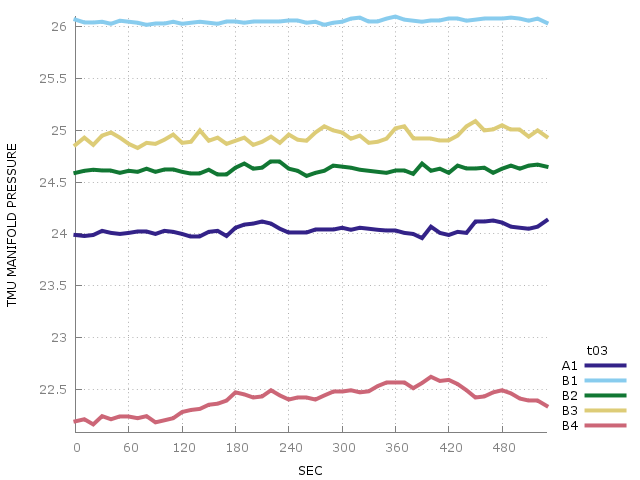
\includegraphics[bb=0 0 640 480, width=5in]{gnu/ld/plot/ManifoldPress_t03.png}}
\caption{Racks A1, B1--4; TMU manifold pressure.}
\end{figure}
\begin{figure}[!h]
\centerline{\bfseries\large Low-Density Workload : Trials 1--3}\\
\fbox{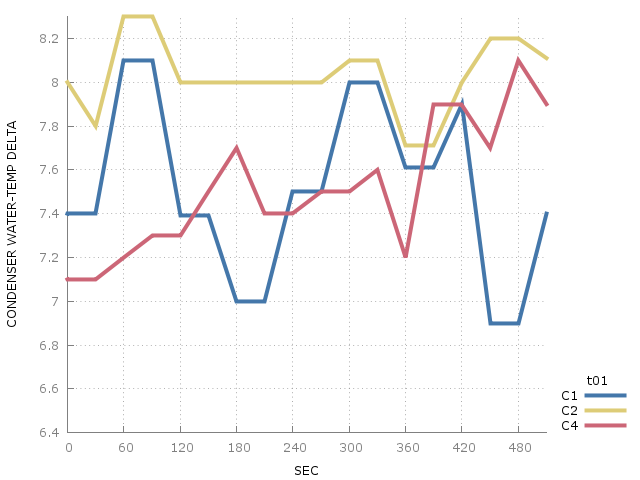
\includegraphics[bb=0 0 640 480, width=5in]{gnu/ld/plot/C_WTD_t01.png}}
\fbox{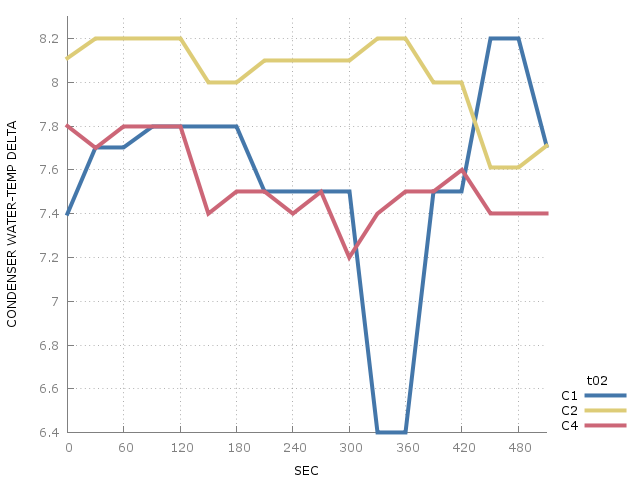
\includegraphics[bb=0 0 640 480, width=5in]{gnu/ld/plot/C_WTD_t02.png}}
\fbox{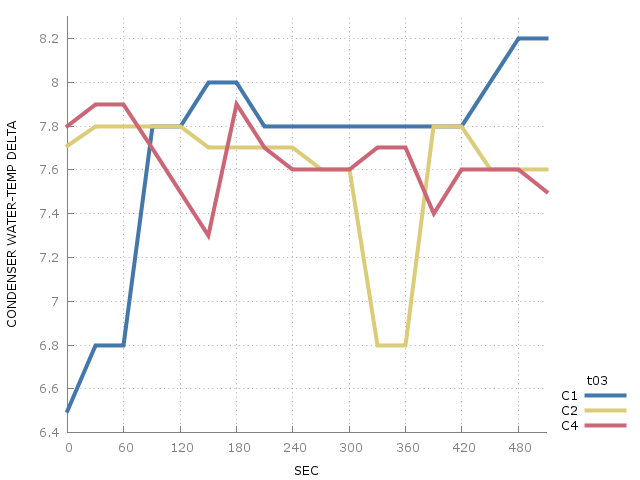
\includegraphics[bb=0 0 640 480, width=5in]{gnu/ld/plot/C_WTD_t03.png}}
\caption{Chillers C1,C2, and C4; Condenser water-temperature delta, which is obtained by subtracting entering from leaving water temperatures ($LCWT-ECWT$).}
\end{figure}
\begin{figure}[!h]
\centerline{\bfseries\large Low-Density Workload : Trials 1--3}\\
\fbox{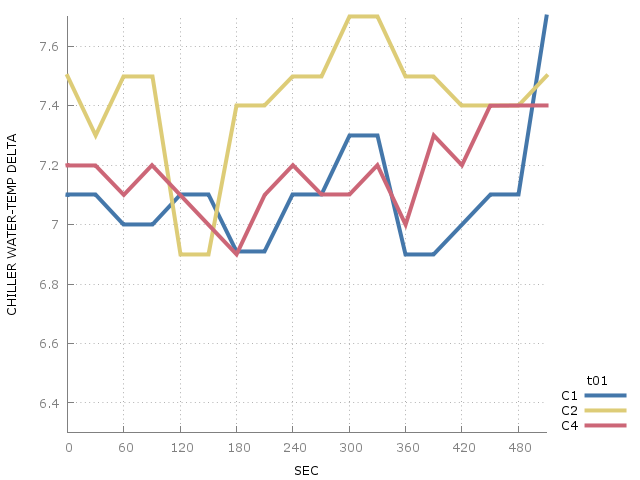
\includegraphics[bb=0 0 640 480, width=5in]{gnu/ld/plot/CH_WTD_t01.png}}
\fbox{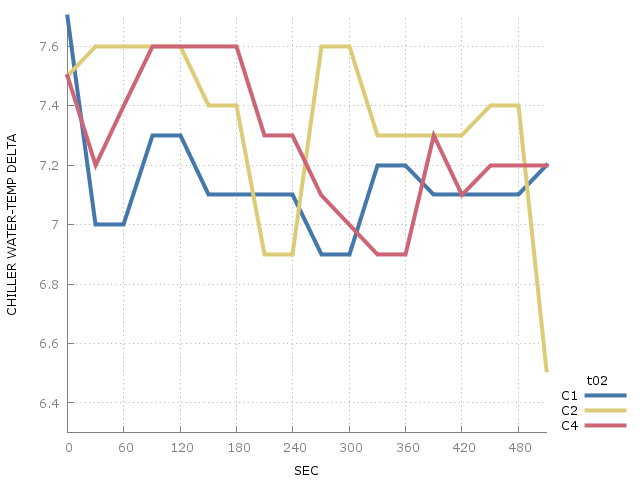
\includegraphics[bb=0 0 640 480, width=5in]{gnu/ld/plot/CH_WTD_t02.png}}
\fbox{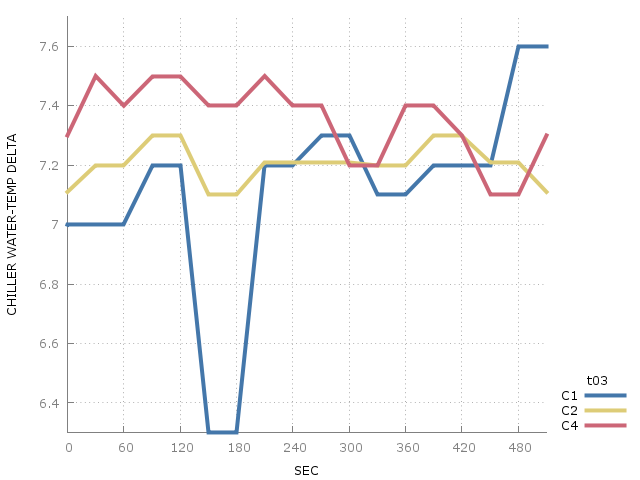
\includegraphics[bb=0 0 640 480, width=5in]{gnu/ld/plot/CH_WTD_t03.png}}
\caption{Chillers C1,C2, and C4; Chilled water-temperature delta, which is obtained by subtracting leaving from entering water temperatures ($ECHWT-LCHWT$).}
\end{figure}
\begin{figure}[!h]
\centerline{\bfseries\large Low-Density Workload : Trials 1--3}\\
\fbox{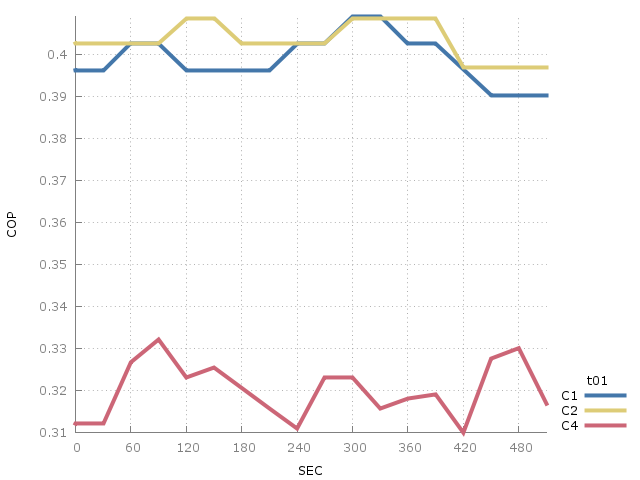
\includegraphics[bb=0 0 640 480, width=5in]{gnu/ld/plot/COP_t01.png}}
\fbox{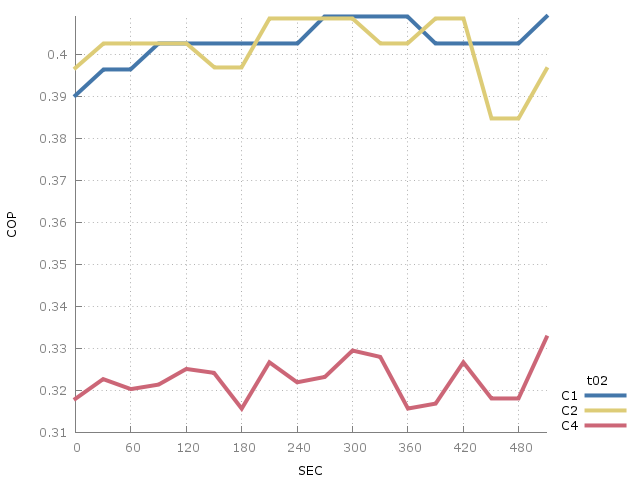
\includegraphics[bb=0 0 640 480, width=5in]{gnu/ld/plot/COP_t02.png}}
\fbox{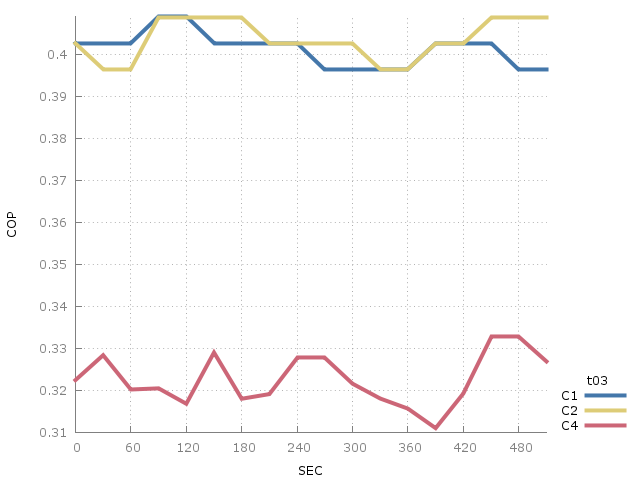
\includegraphics[bb=0 0 640 480, width=5in]{gnu/ld/plot/COP_t03.png}}
\caption{Chillers C1,C2, and C4; Coefficient of performance (COP), which is obtained from dividing Loads by KW.}
\end{figure}
\begin{figure}[!h]
\centerline{\bfseries\large Low-Density Workload : Trials 1--3}\\
\fbox{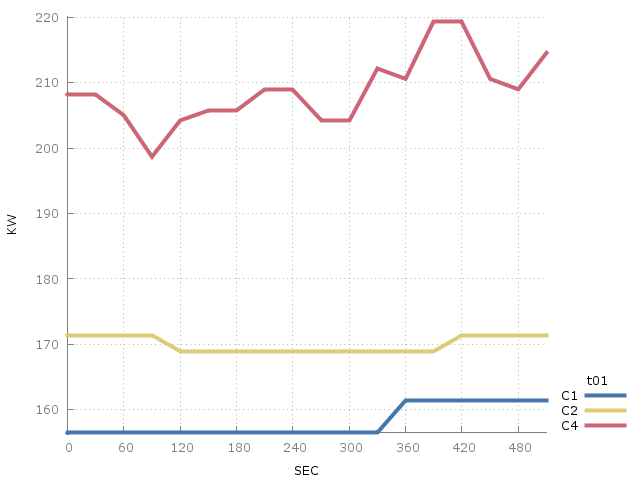
\includegraphics[bb=0 0 640 480, width=5in]{gnu/ld/plot/KW_t01.png}}
\fbox{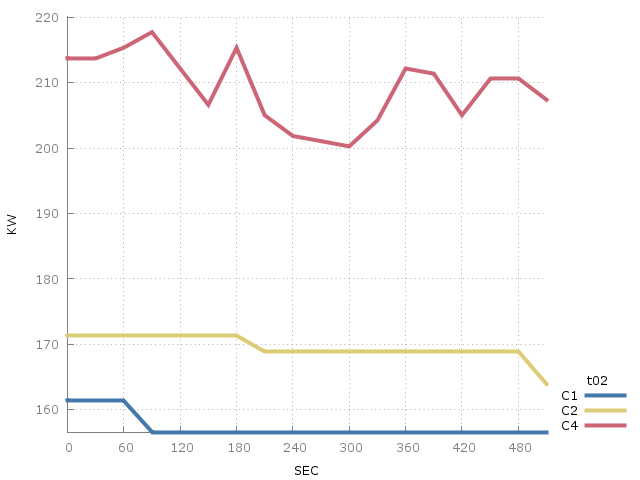
\includegraphics[bb=0 0 640 480, width=5in]{gnu/ld/plot/KW_t02.png}}
\fbox{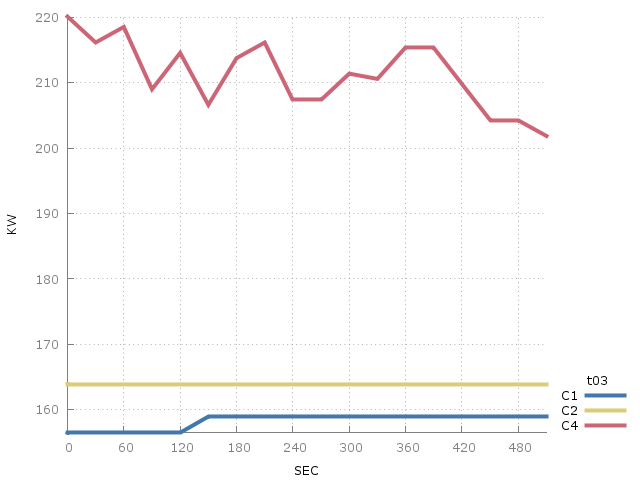
\includegraphics[bb=0 0 640 480, width=5in]{gnu/ld/plot/KW_t03.png}}
\caption{Chillers C1,C2, and C4; Kilowatts (KW). This is the amount of heat that is generated at the data center---approximately equivalent to the power consumed.}
\end{figure}
\begin{figure}[!h]
\centerline{\bfseries\large Low-Density Workload : Trials 1--3}\\
\fbox{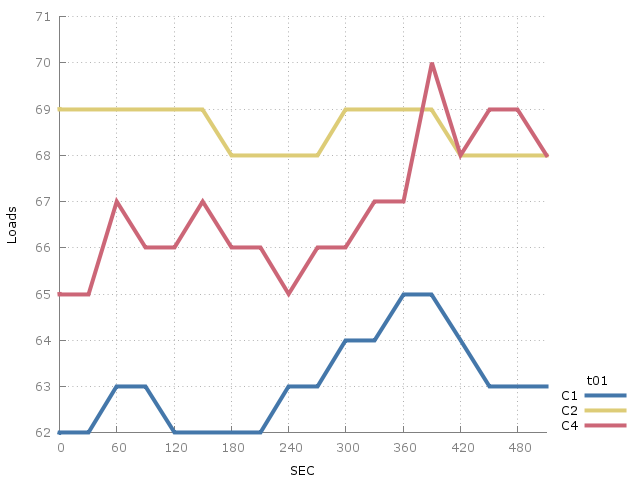
\includegraphics[bb=0 0 640 480, width=5in]{gnu/ld/plot/Loads_t01.png}}
\fbox{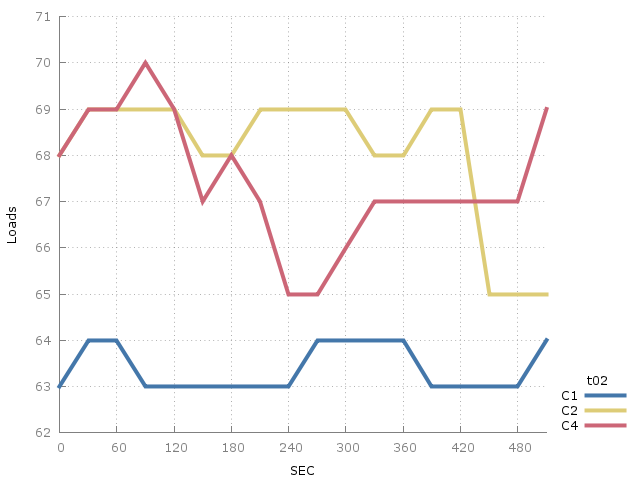
\includegraphics[bb=0 0 640 480, width=5in]{gnu/ld/plot/Loads_t02.png}}
\fbox{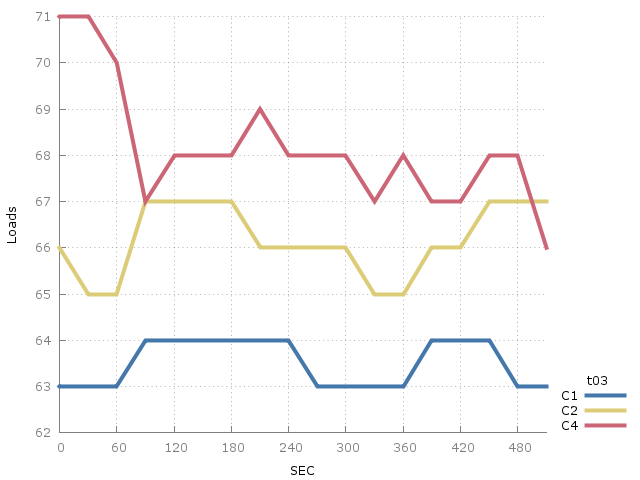
\includegraphics[bb=0 0 640 480, width=5in]{gnu/ld/plot/Loads_t03.png}}
\caption{Chillers C1,C2, and C4; Loads---cooling loads on the chiller units.}
\end{figure}
\chapter{Chiller Metric Clustering : Condenser Water-Temperature Delta}
\begin{figure}[!h]
\centerline{\bfseries\large Low-Density Workload : Trials 1--3}\\
\fbox{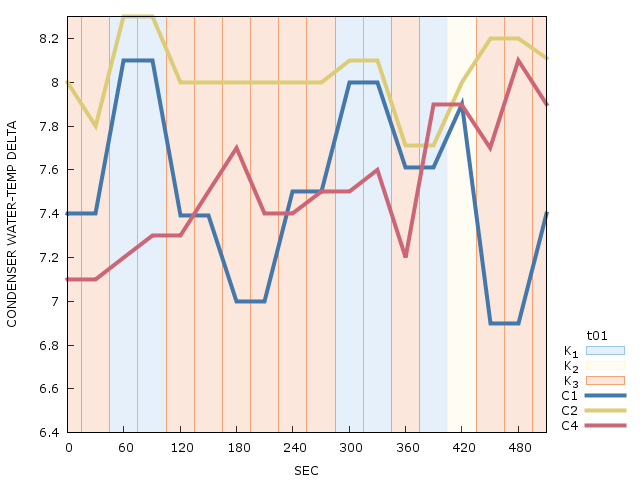
\includegraphics[bb=0 0 640 480, width=5in]{cluster3/ld/C_WTD/C_WTD_t01.png}}
\fbox{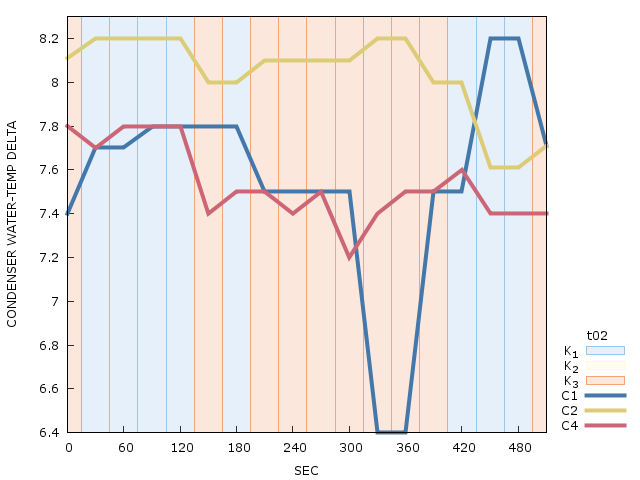
\includegraphics[bb=0 0 640 480, width=5in]{cluster3/ld/C_WTD/C_WTD_t02.png}}
\fbox{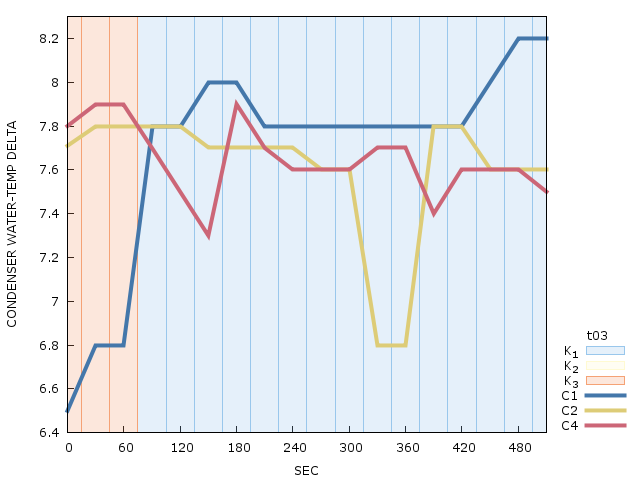
\includegraphics[bb=0 0 640 480, width=5in]{cluster3/ld/C_WTD/C_WTD_t03.png}}
\caption{Chiller units C1, C2, and C4; EM clustering across all three trials with $k=3$.}
\end{figure}
\begin{figure}[!h]
\centerline{\bfseries\large Low-Density Workload : Trials 1--3}\\
\fbox{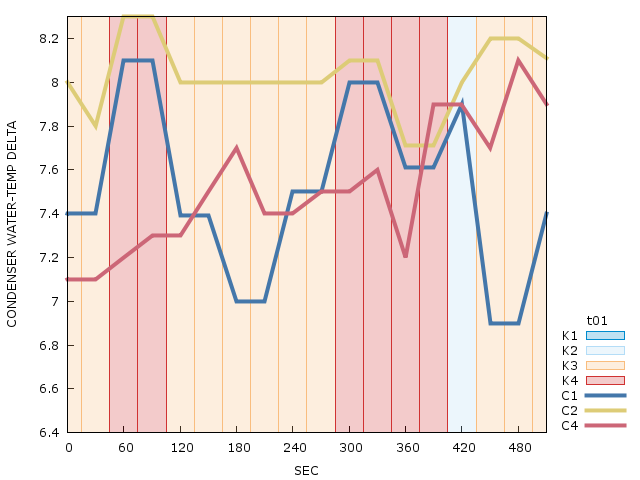
\includegraphics[bb=0 0 640 480, width=5in]{cluster4/ld/C_WTD/C_WTD_t01.png}}
\fbox{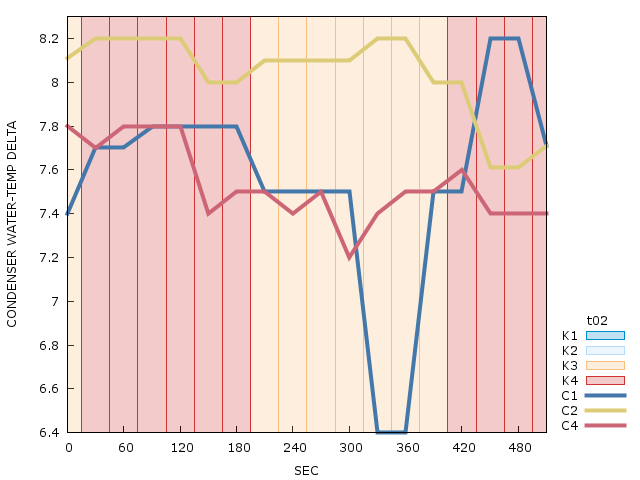
\includegraphics[bb=0 0 640 480, width=5in]{cluster4/ld/C_WTD/C_WTD_t02.png}}
\fbox{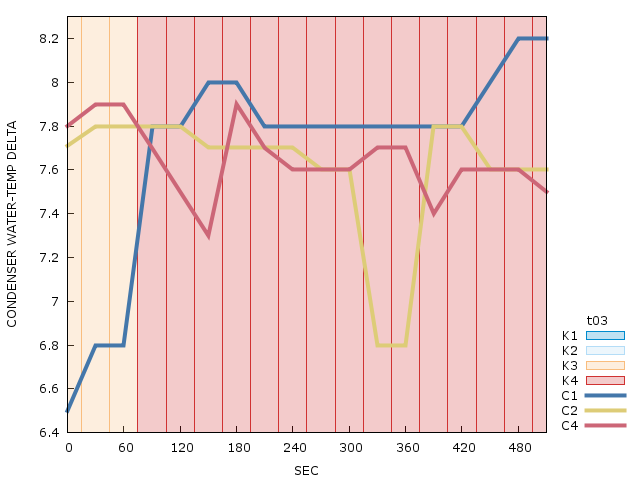
\includegraphics[bb=0 0 640 480, width=5in]{cluster4/ld/C_WTD/C_WTD_t03.png}}
\caption{Chiller units C1, C2, and C4; K-Means clustering across all three trials with $k=4$.}
\end{figure}
\begin{figure}[!h]
\centerline{\bfseries\large Low-Density Workload : Trials 1--3}\\
\fbox{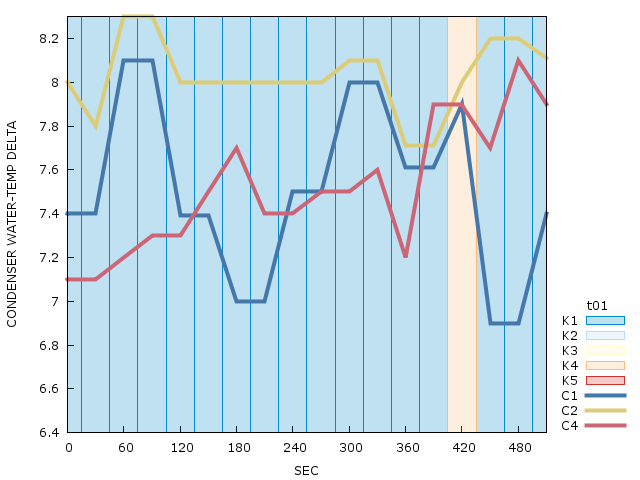
\includegraphics[bb=0 0 640 480, width=5in]{cluster5/ld/C_WTD/C_WTD_t01.png}}
\fbox{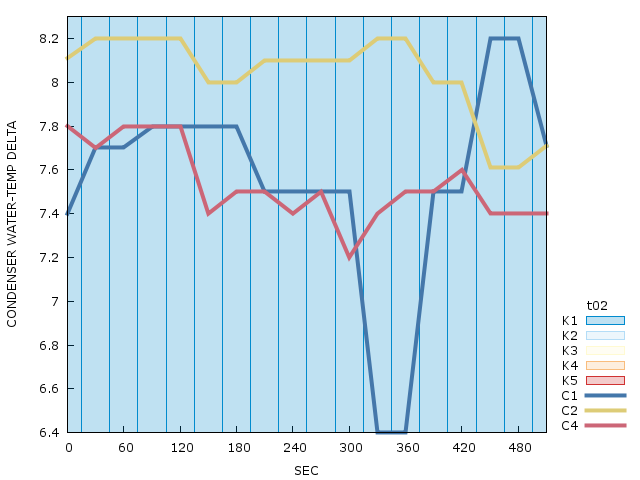
\includegraphics[bb=0 0 640 480, width=5in]{cluster5/ld/C_WTD/C_WTD_t02.png}}
\fbox{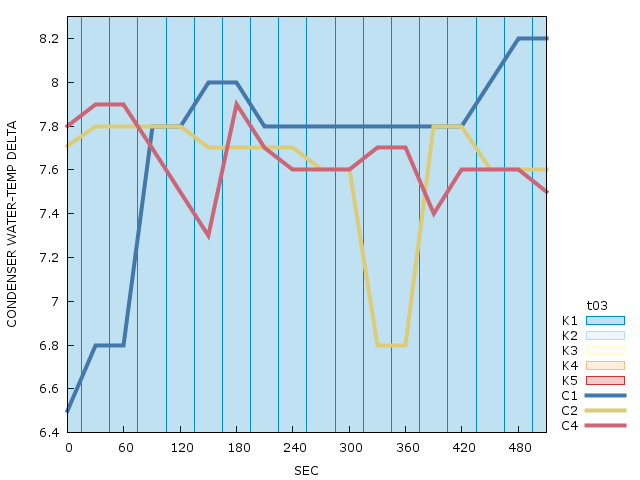
\includegraphics[bb=0 0 640 480, width=5in]{cluster5/ld/C_WTD/C_WTD_t03.png}}
\caption{Chiller units C1, C2, and C4; K-Means clustering across all three trials with $k=5$.}
\end{figure}
\begin{figure}[!h]
\centerline{\bfseries\large Low-Density Workload : Trials 1--3}\\
\fbox{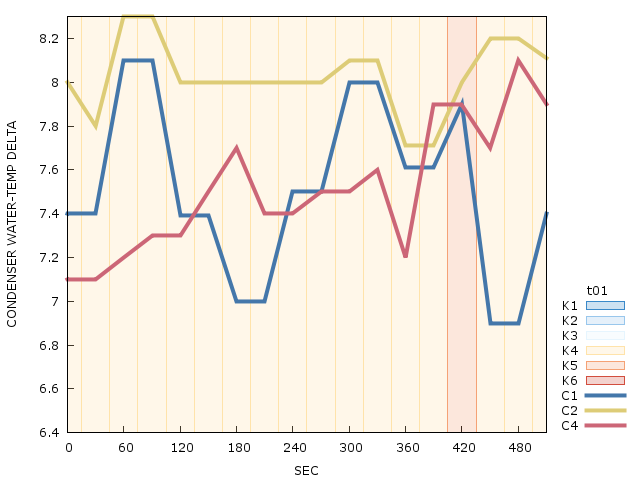
\includegraphics[bb=0 0 640 480, width=5in]{cluster6/ld/C_WTD/C_WTD_t01.png}}
\fbox{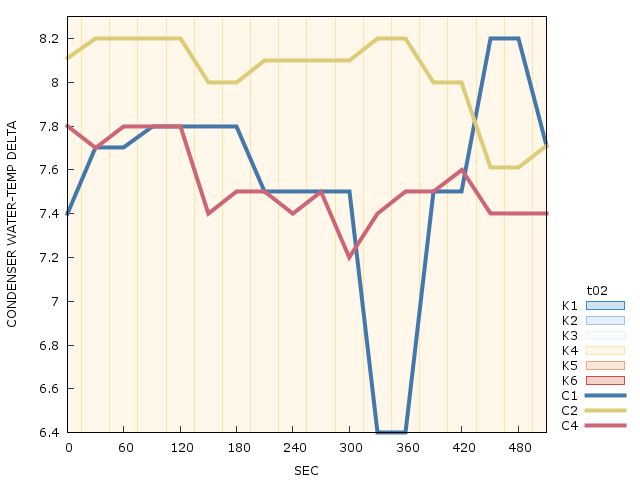
\includegraphics[bb=0 0 640 480, width=5in]{cluster6/ld/C_WTD/C_WTD_t02.png}}
\fbox{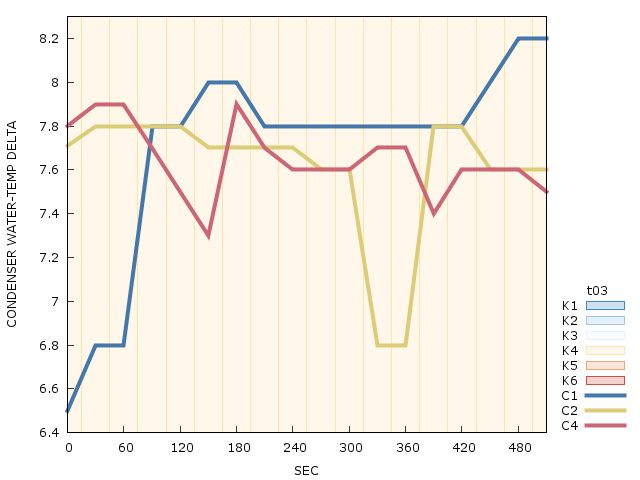
\includegraphics[bb=0 0 640 480, width=5in]{cluster6/ld/C_WTD/C_WTD_t03.png}}
\caption{Chiller units C1, C2, and C4; K-Means clustering across all three trials with $k=6$.}
\end{figure}
\begin{figure}[!h]
\centerline{\bfseries\large Low-Density Workload : Trials 1--3}\\
\fbox{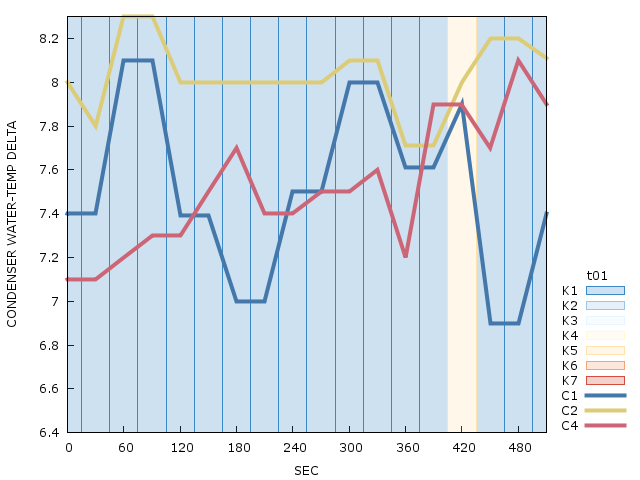
\includegraphics[bb=0 0 640 480, width=5in]{cluster7/ld/C_WTD/C_WTD_t01.png}}
\fbox{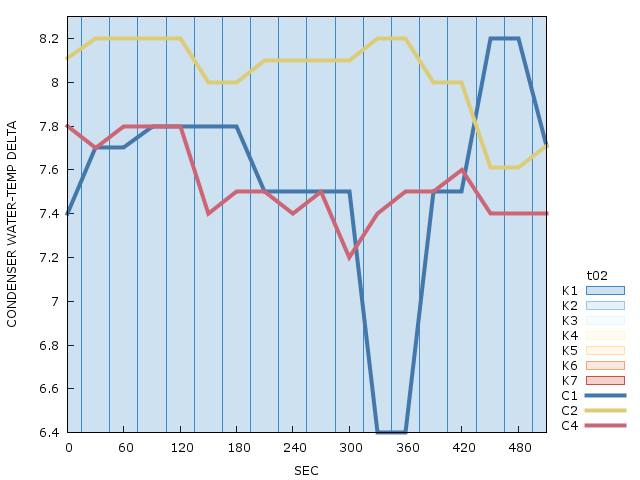
\includegraphics[bb=0 0 640 480, width=5in]{cluster7/ld/C_WTD/C_WTD_t02.png}}
\fbox{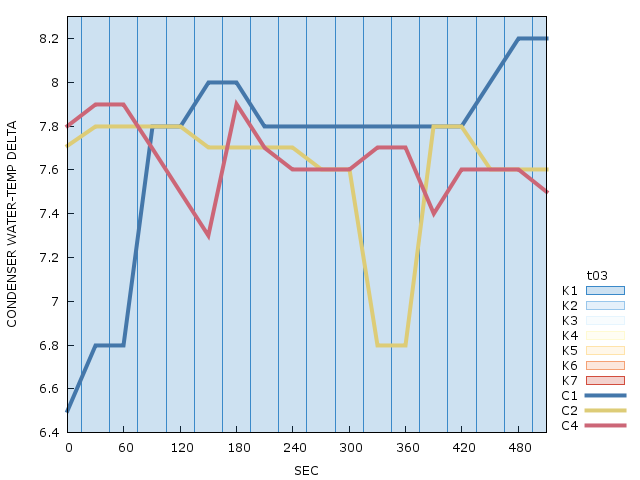
\includegraphics[bb=0 0 640 480, width=5in]{cluster7/ld/C_WTD/C_WTD_t03.png}}
\caption{Chiller units C1, C2, and C4; K-Means clustering across all three trials with $k=7$.}
\end{figure}
\begin{figure}[!h]
\centerline{\bfseries\large Low-Density Workload : Trials 1--3}\\
\fbox{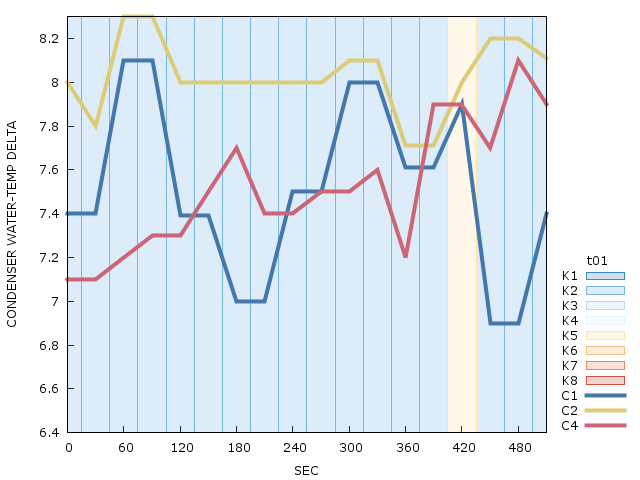
\includegraphics[bb=0 0 640 480, width=5in]{cluster8/ld/C_WTD/C_WTD_t01.png}}
\fbox{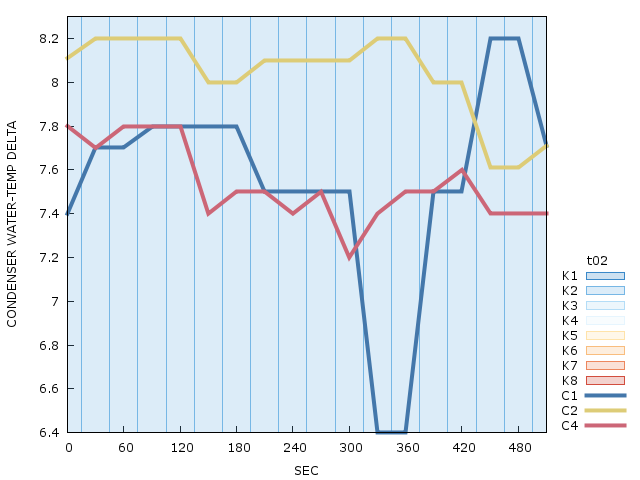
\includegraphics[bb=0 0 640 480, width=5in]{cluster8/ld/C_WTD/C_WTD_t02.png}}
\fbox{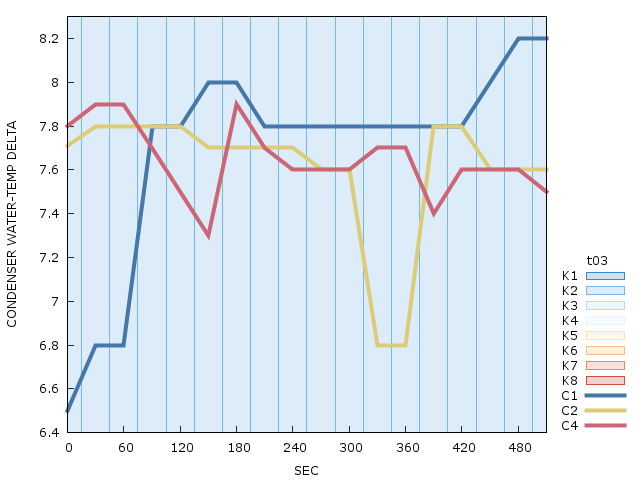
\includegraphics[bb=0 0 640 480, width=5in]{cluster8/ld/C_WTD/C_WTD_t03.png}}
\caption{Chiller units C1, C2, and C4; K-Means clustering across all three trials with $k=8$.}
\end{figure}
\begin{figure}[!h]
\centerline{\bfseries\large Low-Density Workload : Trials 1--3}\\
\fbox{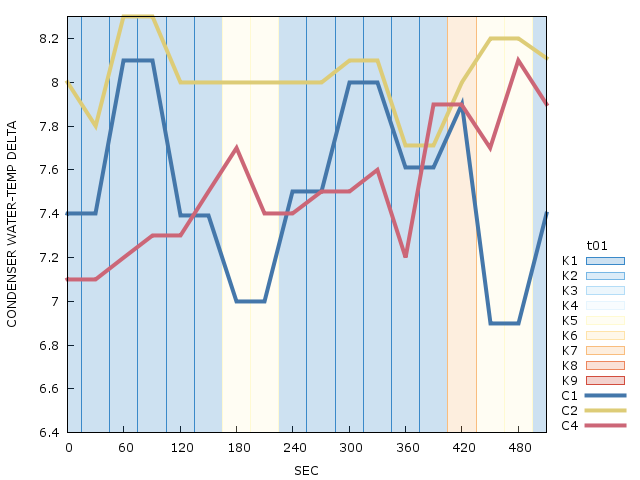
\includegraphics[bb=0 0 640 480, width=5in]{cluster9/ld/C_WTD/C_WTD_t01.png}}
\fbox{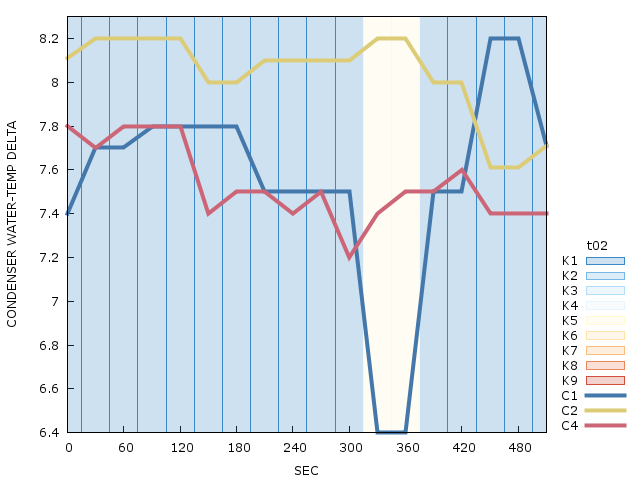
\includegraphics[bb=0 0 640 480, width=5in]{cluster9/ld/C_WTD/C_WTD_t02.png}}
\fbox{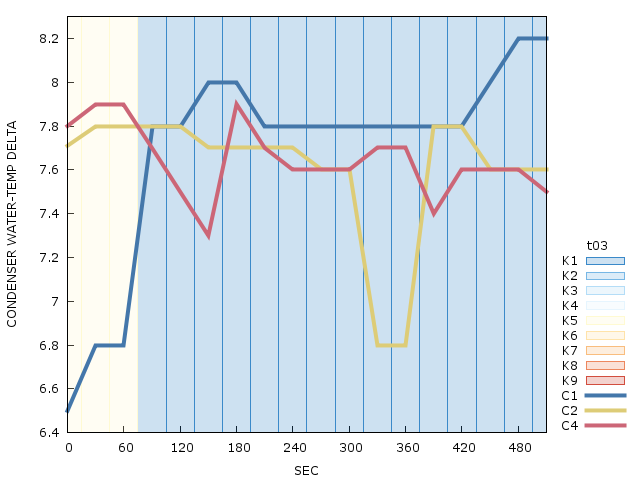
\includegraphics[bb=0 0 640 480, width=5in]{cluster9/ld/C_WTD/C_WTD_t03.png}}
\caption{Chiller units C1, C2, and C4; K-Means clustering across all three trials with $k=9$.}
\end{figure}
\begin{figure}[!h]
\centerline{\bfseries\large Low-Density Workload : Trials 1--3}\\
\fbox{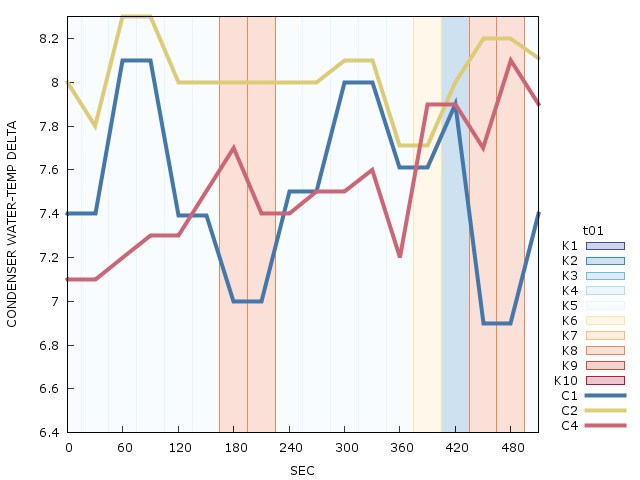
\includegraphics[bb=0 0 640 480, width=5in]{cluster10/ld/C_WTD/C_WTD_t01.png}}
\fbox{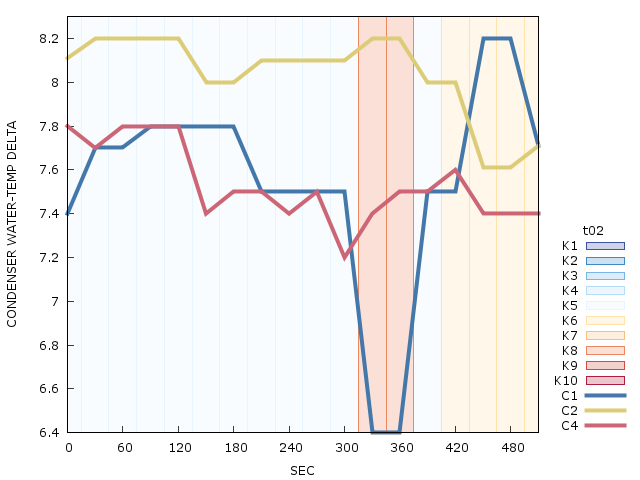
\includegraphics[bb=0 0 640 480, width=5in]{cluster10/ld/C_WTD/C_WTD_t02.png}}
\fbox{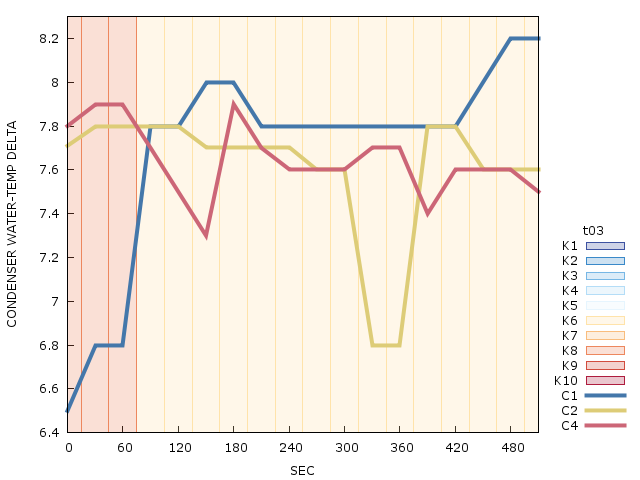
\includegraphics[bb=0 0 640 480, width=5in]{cluster10/ld/C_WTD/C_WTD_t03.png}}
\caption{Chiller units C1, C2, and C4; K-Means clustering across all three trials with $k=10$.}
\end{figure}
\begin{figure}[!h]
\centerline{\bfseries\large Low-Density Workload : Trials 1--3}\\
\fbox{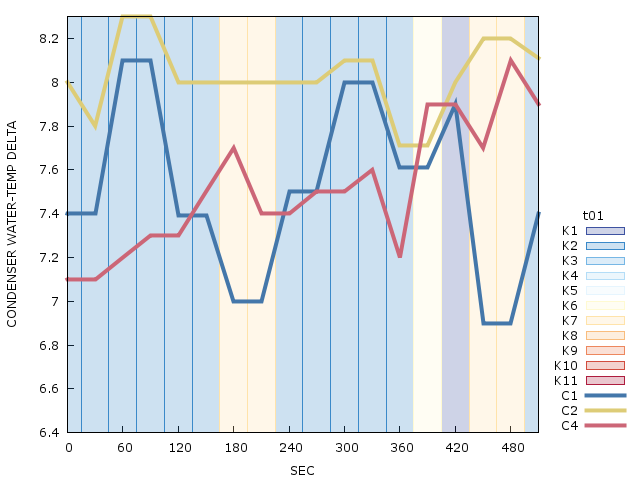
\includegraphics[bb=0 0 640 480, width=5in]{cluster11/ld/C_WTD/C_WTD_t01.png}}
\fbox{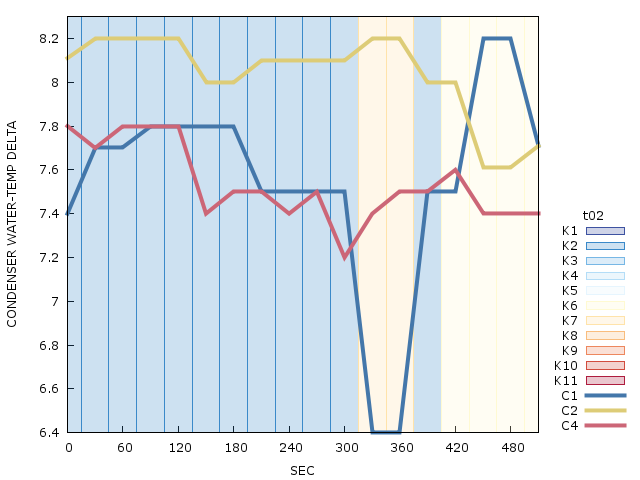
\includegraphics[bb=0 0 640 480, width=5in]{cluster11/ld/C_WTD/C_WTD_t02.png}}
\fbox{\includegraphics[bb=0 0 640 480, width=5in]{cluster11/ld/C_WTD/C_WTD_t03.png}}
\caption{Chiller units C1, C2, and C4; K-Means clustering across all three trials with $k=11$.}
\end{figure}

\chapter{Chiller Metric Clustering : Chilled Water-Temperature Delta}
\begin{figure}[!h]
\centerline{\bfseries\large Low-Density Workload : Trials 1--3}\\
\fbox{\includegraphics[bb=0 0 640 480, width=5in]{cluster3/ld/CH_WTD/CH_WTD_t01.png}}
\fbox{\includegraphics[bb=0 0 640 480, width=5in]{cluster3/ld/CH_WTD/CH_WTD_t02.png}}
\fbox{\includegraphics[bb=0 0 640 480, width=5in]{cluster3/ld/CH_WTD/CH_WTD_t03.png}}
\caption{Chiller units C1, C2, and C4; EM clustering across all three trials with $k=3$.}
\end{figure}
\begin{figure}[!h]
\centerline{\bfseries\large Low-Density Workload : Trials 1--3}\\
\fbox{\includegraphics[bb=0 0 640 480, width=5in]{cluster4/ld/CH_WTD/CH_WTD_t01.png}}
\fbox{\includegraphics[bb=0 0 640 480, width=5in]{cluster4/ld/CH_WTD/CH_WTD_t02.png}}
\fbox{\includegraphics[bb=0 0 640 480, width=5in]{cluster4/ld/CH_WTD/CH_WTD_t03.png}}
\caption{Chiller units C1, C2, and C4; K-Means clustering across all three trials with $k=4$.}
\end{figure}
\begin{figure}[!h]
\centerline{\bfseries\large Low-Density Workload : Trials 1--3}\\
\fbox{\includegraphics[bb=0 0 640 480, width=5in]{cluster5/ld/CH_WTD/CH_WTD_t01.png}}
\fbox{\includegraphics[bb=0 0 640 480, width=5in]{cluster5/ld/CH_WTD/CH_WTD_t02.png}}
\fbox{\includegraphics[bb=0 0 640 480, width=5in]{cluster5/ld/CH_WTD/CH_WTD_t03.png}}
\caption{Chiller units C1, C2, and C4; K-Means clustering across all three trials with $k=5$.}
\end{figure}
\begin{figure}[!h]
\centerline{\bfseries\large Low-Density Workload : Trials 1--3}\\
\fbox{\includegraphics[bb=0 0 640 480, width=5in]{cluster6/ld/CH_WTD/CH_WTD_t01.png}}
\fbox{\includegraphics[bb=0 0 640 480, width=5in]{cluster6/ld/CH_WTD/CH_WTD_t02.png}}
\fbox{\includegraphics[bb=0 0 640 480, width=5in]{cluster6/ld/CH_WTD/CH_WTD_t03.png}}
\caption{Chiller units C1, C2, and C4; K-Means clustering across all three trials with $k=6$.}
\end{figure}
\begin{figure}[!h]
\centerline{\bfseries\large Low-Density Workload : Trials 1--3}\\
\fbox{\includegraphics[bb=0 0 640 480, width=5in]{cluster7/ld/CH_WTD/CH_WTD_t01.png}}
\fbox{\includegraphics[bb=0 0 640 480, width=5in]{cluster7/ld/CH_WTD/CH_WTD_t02.png}}
\fbox{\includegraphics[bb=0 0 640 480, width=5in]{cluster7/ld/CH_WTD/CH_WTD_t03.png}}
\caption{Chiller units C1, C2, and C4; K-Means clustering across all three trials with $k=7$.}
\end{figure}
\begin{figure}[!h]
\centerline{\bfseries\large Low-Density Workload : Trials 1--3}\\
\fbox{\includegraphics[bb=0 0 640 480, width=5in]{cluster8/ld/CH_WTD/CH_WTD_t01.png}}
\fbox{\includegraphics[bb=0 0 640 480, width=5in]{cluster8/ld/CH_WTD/CH_WTD_t02.png}}
\fbox{\includegraphics[bb=0 0 640 480, width=5in]{cluster8/ld/CH_WTD/CH_WTD_t03.png}}
\caption{Chiller units C1, C2, and C4; K-Means clustering across all three trials with $k=8$.}
\end{figure}
\begin{figure}[!h]
\centerline{\bfseries\large Low-Density Workload : Trials 1--3}\\
\fbox{\includegraphics[bb=0 0 640 480, width=5in]{cluster9/ld/CH_WTD/CH_WTD_t01.png}}
\fbox{\includegraphics[bb=0 0 640 480, width=5in]{cluster9/ld/CH_WTD/CH_WTD_t02.png}}
\fbox{\includegraphics[bb=0 0 640 480, width=5in]{cluster9/ld/CH_WTD/CH_WTD_t03.png}}
\caption{Chiller units C1, C2, and C4; K-Means clustering across all three trials with $k=9$.}
\end{figure}
\begin{figure}[!h]
\centerline{\bfseries\large Low-Density Workload : Trials 1--3}\\
\fbox{\includegraphics[bb=0 0 640 480, width=5in]{cluster10/ld/CH_WTD/CH_WTD_t01.png}}
\fbox{\includegraphics[bb=0 0 640 480, width=5in]{cluster10/ld/CH_WTD/CH_WTD_t02.png}}
\fbox{\includegraphics[bb=0 0 640 480, width=5in]{cluster10/ld/CH_WTD/CH_WTD_t03.png}}
\caption{Chiller units C1, C2, and C4; K-Means clustering across all three trials with $k=10$.}
\end{figure}
\begin{figure}[!h]
\centerline{\bfseries\large Low-Density Workload : Trials 1--3}\\
\fbox{\includegraphics[bb=0 0 640 480, width=5in]{cluster11/ld/CH_WTD/CH_WTD_t01.png}}
\fbox{\includegraphics[bb=0 0 640 480, width=5in]{cluster11/ld/CH_WTD/CH_WTD_t02.png}}
\fbox{\includegraphics[bb=0 0 640 480, width=5in]{cluster11/ld/CH_WTD/CH_WTD_t03.png}}
\caption{Chiller units C1, C2, and C4; K-Means clustering across all three trials with $k=11$.}
\end{figure}

\chapter{Chiller Metric Clustering : Coefficient of Performance (COP)}
\begin{figure}[!h]
\centerline{\bfseries\large Low-Density Workload : Trials 1--3}\\
\fbox{\includegraphics[bb=0 0 640 480, width=5in]{cluster3/ld/COP/COP_t01.png}}
\fbox{\includegraphics[bb=0 0 640 480, width=5in]{cluster3/ld/COP/COP_t02.png}}
\fbox{\includegraphics[bb=0 0 640 480, width=5in]{cluster3/ld/COP/COP_t03.png}}
\caption{Chiller units C1, C2, and C4; EM clustering across all three trials with $k=3$.}
\end{figure}
\begin{figure}[!h]
\centerline{\bfseries\large Low-Density Workload : Trials 1--3}\\
\fbox{\includegraphics[bb=0 0 640 480, width=5in]{cluster4/ld/COP/COP_t01.png}}
\fbox{\includegraphics[bb=0 0 640 480, width=5in]{cluster4/ld/COP/COP_t02.png}}
\fbox{\includegraphics[bb=0 0 640 480, width=5in]{cluster4/ld/COP/COP_t03.png}}
\caption{Chiller units C1, C2, and C4; K-Means clustering across all three trials with $k=4$.}
\end{figure}
\begin{figure}[!h]
\centerline{\bfseries\large Low-Density Workload : Trials 1--3}\\
\fbox{\includegraphics[bb=0 0 640 480, width=5in]{cluster5/ld/COP/COP_t01.png}}
\fbox{\includegraphics[bb=0 0 640 480, width=5in]{cluster5/ld/COP/COP_t02.png}}
\fbox{\includegraphics[bb=0 0 640 480, width=5in]{cluster5/ld/COP/COP_t03.png}}
\caption{Chiller units C1, C2, and C4; K-Means clustering across all three trials with $k=5$.}
\end{figure}
\begin{figure}[!h]
\centerline{\bfseries\large Low-Density Workload : Trials 1--3}\\
\fbox{\includegraphics[bb=0 0 640 480, width=5in]{cluster6/ld/COP/COP_t01.png}}
\fbox{\includegraphics[bb=0 0 640 480, width=5in]{cluster6/ld/COP/COP_t02.png}}
\fbox{\includegraphics[bb=0 0 640 480, width=5in]{cluster6/ld/COP/COP_t03.png}}
\caption{Chiller units C1, C2, and C4; K-Means clustering across all three trials with $k=6$.}
\end{figure}
\begin{figure}[!h]
\centerline{\bfseries\large Low-Density Workload : Trials 1--3}\\
\fbox{\includegraphics[bb=0 0 640 480, width=5in]{cluster7/ld/COP/COP_t01.png}}
\fbox{\includegraphics[bb=0 0 640 480, width=5in]{cluster7/ld/COP/COP_t02.png}}
\fbox{\includegraphics[bb=0 0 640 480, width=5in]{cluster7/ld/COP/COP_t03.png}}
\caption{Chiller units C1, C2, and C4; K-Means clustering across all three trials with $k=7$.}
\end{figure}
\begin{figure}[!h]
\centerline{\bfseries\large Low-Density Workload : Trials 1--3}\\
\fbox{\includegraphics[bb=0 0 640 480, width=5in]{cluster8/ld/COP/COP_t01.png}}
\fbox{\includegraphics[bb=0 0 640 480, width=5in]{cluster8/ld/COP/COP_t02.png}}
\fbox{\includegraphics[bb=0 0 640 480, width=5in]{cluster8/ld/COP/COP_t03.png}}
\caption{Chiller units C1, C2, and C4; K-Means clustering across all three trials with $k=8$.}
\end{figure}
\begin{figure}[!h]
\centerline{\bfseries\large Low-Density Workload : Trials 1--3}\\
\fbox{\includegraphics[bb=0 0 640 480, width=5in]{cluster9/ld/COP/COP_t01.png}}
\fbox{\includegraphics[bb=0 0 640 480, width=5in]{cluster9/ld/COP/COP_t02.png}}
\fbox{\includegraphics[bb=0 0 640 480, width=5in]{cluster9/ld/COP/COP_t03.png}}
\caption{Chiller units C1, C2, and C4; K-Means clustering across all three trials with $k=9$.}
\end{figure}
\begin{figure}[!h]
\centerline{\bfseries\large Low-Density Workload : Trials 1--3}\\
\fbox{\includegraphics[bb=0 0 640 480, width=5in]{cluster10/ld/COP/COP_t01.png}}
\fbox{\includegraphics[bb=0 0 640 480, width=5in]{cluster10/ld/COP/COP_t02.png}}
\fbox{\includegraphics[bb=0 0 640 480, width=5in]{cluster10/ld/COP/COP_t03.png}}
\caption{Chiller units C1, C2, and C4; K-Means clustering across all three trials with $k=10$.}
\end{figure}
\begin{figure}[!h]
\centerline{\bfseries\large Low-Density Workload : Trials 1--3}\\
\fbox{\includegraphics[bb=0 0 640 480, width=5in]{cluster11/ld/COP/COP_t01.png}}
\fbox{\includegraphics[bb=0 0 640 480, width=5in]{cluster11/ld/COP/COP_t02.png}}
\fbox{\includegraphics[bb=0 0 640 480, width=5in]{cluster11/ld/COP/COP_t03.png}}
\caption{Chiller units C1, C2, and C4; K-Means clustering across all three trials with $k=11$.}
\end{figure}

\chapter{Chiller Metric Clustering : KW}
\begin{figure}[!h]
\centerline{\bfseries\large Low-Density Workload : Trials 1--3}\\
\fbox{\includegraphics[bb=0 0 640 480, width=5in]{cluster3/ld/KW/KW_t01.png}}
\fbox{\includegraphics[bb=0 0 640 480, width=5in]{cluster3/ld/KW/KW_t02.png}}
\fbox{\includegraphics[bb=0 0 640 480, width=5in]{cluster3/ld/KW/KW_t03.png}}
\caption{Chiller units C1, C2, and C4; EM clustering across all three trials with $k=3$.}
\end{figure}
\begin{figure}[!h]
\centerline{\bfseries\large Low-Density Workload : Trials 1--3}\\
\fbox{\includegraphics[bb=0 0 640 480, width=5in]{cluster4/ld/KW/KW_t01.png}}
\fbox{\includegraphics[bb=0 0 640 480, width=5in]{cluster4/ld/KW/KW_t02.png}}
\fbox{\includegraphics[bb=0 0 640 480, width=5in]{cluster4/ld/KW/KW_t03.png}}
\caption{Chiller units C1, C2, and C4; K-Means clustering across all three trials with $k=4$.}
\end{figure}
\begin{figure}[!h]
\centerline{\bfseries\large Low-Density Workload : Trials 1--3}\\
\fbox{\includegraphics[bb=0 0 640 480, width=5in]{cluster5/ld/KW/KW_t01.png}}
\fbox{\includegraphics[bb=0 0 640 480, width=5in]{cluster5/ld/KW/KW_t02.png}}
\fbox{\includegraphics[bb=0 0 640 480, width=5in]{cluster5/ld/KW/KW_t03.png}}
\caption{Chiller units C1, C2, and C4; K-Means clustering across all three trials with $k=5$.}
\end{figure}
\begin{figure}[!h]
\centerline{\bfseries\large Low-Density Workload : Trials 1--3}\\
\fbox{\includegraphics[bb=0 0 640 480, width=5in]{cluster6/ld/KW/KW_t01.png}}
\fbox{\includegraphics[bb=0 0 640 480, width=5in]{cluster6/ld/KW/KW_t02.png}}
\fbox{\includegraphics[bb=0 0 640 480, width=5in]{cluster6/ld/KW/KW_t03.png}}
\caption{Chiller units C1, C2, and C4; K-Means clustering across all three trials with $k=6$.}
\end{figure}
\begin{figure}[!h]
\centerline{\bfseries\large Low-Density Workload : Trials 1--3}\\
\fbox{\includegraphics[bb=0 0 640 480, width=5in]{cluster7/ld/KW/KW_t01.png}}
\fbox{\includegraphics[bb=0 0 640 480, width=5in]{cluster7/ld/KW/KW_t02.png}}
\fbox{\includegraphics[bb=0 0 640 480, width=5in]{cluster7/ld/KW/KW_t03.png}}
\caption{Chiller units C1, C2, and C4; K-Means clustering across all three trials with $k=7$.}
\end{figure}
\begin{figure}[!h]
\centerline{\bfseries\large Low-Density Workload : Trials 1--3}\\
\fbox{\includegraphics[bb=0 0 640 480, width=5in]{cluster8/ld/KW/KW_t01.png}}
\fbox{\includegraphics[bb=0 0 640 480, width=5in]{cluster8/ld/KW/KW_t02.png}}
\fbox{\includegraphics[bb=0 0 640 480, width=5in]{cluster8/ld/KW/KW_t03.png}}
\caption{Chiller units C1, C2, and C4; K-Means clustering across all three trials with $k=8$.}
\end{figure}
\begin{figure}[!h]
\centerline{\bfseries\large Low-Density Workload : Trials 1--3}\\
\fbox{\includegraphics[bb=0 0 640 480, width=5in]{cluster9/ld/KW/KW_t01.png}}
\fbox{\includegraphics[bb=0 0 640 480, width=5in]{cluster9/ld/KW/KW_t02.png}}
\fbox{\includegraphics[bb=0 0 640 480, width=5in]{cluster9/ld/KW/KW_t03.png}}
\caption{Chiller units C1, C2, and C4; K-Means clustering across all three trials with $k=9$.}
\end{figure}
\begin{figure}[!h]
\centerline{\bfseries\large Low-Density Workload : Trials 1--3}\\
\fbox{\includegraphics[bb=0 0 640 480, width=5in]{cluster10/ld/KW/KW_t01.png}}
\fbox{\includegraphics[bb=0 0 640 480, width=5in]{cluster10/ld/KW/KW_t02.png}}
\fbox{\includegraphics[bb=0 0 640 480, width=5in]{cluster10/ld/KW/KW_t03.png}}
\caption{Chiller units C1, C2, and C4; K-Means clustering across all three trials with $k=10$.}
\end{figure}
\begin{figure}[!h]
\centerline{\bfseries\large Low-Density Workload : Trials 1--3}\\
\fbox{\includegraphics[bb=0 0 640 480, width=5in]{cluster11/ld/KW/KW_t01.png}}
\fbox{\includegraphics[bb=0 0 640 480, width=5in]{cluster11/ld/KW/KW_t02.png}}
\fbox{\includegraphics[bb=0 0 640 480, width=5in]{cluster11/ld/KW/KW_t03.png}}
\caption{Chiller units C1, C2, and C4; K-Means clustering across all three trials with $k=11$.}
\end{figure}

\chapter{Chiller Metric Clustering : Loads}
\begin{figure}[!h]
\centerline{\bfseries\large Low-Density Workload : Trials 1--3}\\
\fbox{\includegraphics[bb=0 0 640 480, width=5in]{cluster3/ld/Loads/Loads_t01.png}}
\fbox{\includegraphics[bb=0 0 640 480, width=5in]{cluster3/ld/Loads/Loads_t02.png}}
\fbox{\includegraphics[bb=0 0 640 480, width=5in]{cluster3/ld/Loads/Loads_t03.png}}
\caption{Chiller units C1, C2, and C4; EM clustering across all three trials with $k=3$.}
\end{figure}
\begin{figure}[!h]
\centerline{\bfseries\large Low-Density Workload : Trials 1--3}\\
\fbox{\includegraphics[bb=0 0 640 480, width=5in]{cluster4/ld/Loads/Loads_t01.png}}
\fbox{\includegraphics[bb=0 0 640 480, width=5in]{cluster4/ld/Loads/Loads_t02.png}}
\fbox{\includegraphics[bb=0 0 640 480, width=5in]{cluster4/ld/Loads/Loads_t03.png}}
\caption{Chiller units C1, C2, and C4; K-Means clustering across all three trials with $k=4$.}
\end{figure}
\begin{figure}[!h]
\centerline{\bfseries\large Low-Density Workload : Trials 1--3}\\
\fbox{\includegraphics[bb=0 0 640 480, width=5in]{cluster5/ld/Loads/Loads_t01.png}}
\fbox{\includegraphics[bb=0 0 640 480, width=5in]{cluster5/ld/Loads/Loads_t02.png}}
\fbox{\includegraphics[bb=0 0 640 480, width=5in]{cluster5/ld/Loads/Loads_t03.png}}
\caption{Chiller units C1, C2, and C4; K-Means clustering across all three trials with $k=5$.}
\end{figure}
\begin{figure}[!h]
\centerline{\bfseries\large Low-Density Workload : Trials 1--3}\\
\fbox{\includegraphics[bb=0 0 640 480, width=5in]{cluster6/ld/Loads/Loads_t01.png}}
\fbox{\includegraphics[bb=0 0 640 480, width=5in]{cluster6/ld/Loads/Loads_t02.png}}
\fbox{\includegraphics[bb=0 0 640 480, width=5in]{cluster6/ld/Loads/Loads_t03.png}}
\caption{Chiller units C1, C2, and C4; K-Means clustering across all three trials with $k=6$.}
\end{figure}
\begin{figure}[!h]
\centerline{\bfseries\large Low-Density Workload : Trials 1--3}\\
\fbox{\includegraphics[bb=0 0 640 480, width=5in]{cluster7/ld/Loads/Loads_t01.png}}
\fbox{\includegraphics[bb=0 0 640 480, width=5in]{cluster7/ld/Loads/Loads_t02.png}}
\fbox{\includegraphics[bb=0 0 640 480, width=5in]{cluster7/ld/Loads/Loads_t03.png}}
\caption{Chiller units C1, C2, and C4; K-Means clustering across all three trials with $k=7$.}
\end{figure}
\begin{figure}[!h]
\centerline{\bfseries\large Low-Density Workload : Trials 1--3}\\
\fbox{\includegraphics[bb=0 0 640 480, width=5in]{cluster8/ld/Loads/Loads_t01.png}}
\fbox{\includegraphics[bb=0 0 640 480, width=5in]{cluster8/ld/Loads/Loads_t02.png}}
\fbox{\includegraphics[bb=0 0 640 480, width=5in]{cluster8/ld/Loads/Loads_t03.png}}
\caption{Chiller units C1, C2, and C4; K-Means clustering across all three trials with $k=8$.}
\end{figure}
\begin{figure}[!h]
\centerline{\bfseries\large Low-Density Workload : Trials 1--3}\\
\fbox{\includegraphics[bb=0 0 640 480, width=5in]{cluster9/ld/Loads/Loads_t01.png}}
\fbox{\includegraphics[bb=0 0 640 480, width=5in]{cluster9/ld/Loads/Loads_t02.png}}
\fbox{\includegraphics[bb=0 0 640 480, width=5in]{cluster9/ld/Loads/Loads_t03.png}}
\caption{Chiller units C1, C2, and C4; K-Means clustering across all three trials with $k=9$.}
\end{figure}
\begin{figure}[!h]
\centerline{\bfseries\large Low-Density Workload : Trials 1--3}\\
\fbox{\includegraphics[bb=0 0 640 480, width=5in]{cluster10/ld/Loads/Loads_t01.png}}
\fbox{\includegraphics[bb=0 0 640 480, width=5in]{cluster10/ld/Loads/Loads_t02.png}}
\fbox{\includegraphics[bb=0 0 640 480, width=5in]{cluster10/ld/Loads/Loads_t03.png}}
\caption{Chiller units C1, C2, and C4; K-Means clustering across all three trials with $k=10$.}
\end{figure}
\begin{figure}[!h]
\centerline{\bfseries\large Low-Density Workload : Trials 1--3}\\
\fbox{\includegraphics[bb=0 0 640 480, width=5in]{cluster11/ld/Loads/Loads_t01.png}}
\fbox{\includegraphics[bb=0 0 640 480, width=5in]{cluster11/ld/Loads/Loads_t02.png}}
\fbox{\includegraphics[bb=0 0 640 480, width=5in]{cluster11/ld/Loads/Loads_t03.png}}
\caption{Chiller units C1, C2, and C4; K-Means clustering across all three trials with $k=11$.}
\end{figure}

\part{High-Density Workload Visualizations}
\chapter{Metrics : Power Unit and Chiller}
\begin{figure}[!h]
\centerline{\bfseries\large High-Density Workload : Trials 1--3}\\
\fbox{\includegraphics[bb=0 0 1152 720, width=15in]{gnu/hd/plot/PowerKWH_t01.png}}
\fbox{\includegraphics[bb=0 0 1152 720, width=15in]{gnu/hd/plot/PowerKWH_t02.png}}
\fbox{\includegraphics[bb=0 0 1152 720, width=15in]{gnu/hd/plot/PowerKWH_t03.png}}
\caption{Racks A1, A3, A4, B1--4; Power-unit kWh increase (7.63\textcent{} per kWh, in Oregon).}
\end{figure}
\begin{figure}[!h]
\centerline{\bfseries\large High-Density Workload : Trials 1--3}\\
\fbox{\includegraphics[bb=0 0 1152 720, width=15in]{gnu/hd/plot/C_WTD_t01.png}}
\fbox{\includegraphics[bb=0 0 1152 720, width=15in]{gnu/hd/plot/C_WTD_t02.png}}
\fbox{\includegraphics[bb=0 0 1152 720, width=15in]{gnu/hd/plot/C_WTD_t03.png}}
\caption{Chillers C1 and C4; Condenser water-temperature delta, which is obtained by subtracting entering from leaving water temperatures ($LCWT-ECWT$).}
\end{figure}
\begin{figure}[!h]
\centerline{\bfseries\large High-Density Workload : Trials 1--3}\\
\fbox{\includegraphics[bb=0 0 1152 720, width=15in]{gnu/hd/plot/CH_WTD_t01.png}}
\fbox{\includegraphics[bb=0 0 1152 720, width=15in]{gnu/hd/plot/CH_WTD_t02.png}}
\fbox{\includegraphics[bb=0 0 1152 720, width=15in]{gnu/hd/plot/CH_WTD_t03.png}}
\caption{Chillers C1 and C4; Chilled water-temperature delta, which is obtained by subtracting leaving from entering water temperatures ($ECHWT-LCHWT$).}
\end{figure}
\begin{figure}[!h]
\centerline{\bfseries\large High-Density Workload : Trials 1--3}\\
\fbox{\includegraphics[bb=0 0 1152 720, width=15in]{gnu/hd/plot/COP_t01.png}}
\fbox{\includegraphics[bb=0 0 1152 720, width=15in]{gnu/hd/plot/COP_t02.png}}
\fbox{\includegraphics[bb=0 0 1152 720, width=15in]{gnu/hd/plot/COP_t03.png}}
\caption{Chillers C1 and C4; Coefficient of performance (COP), which is obtained from dividing Loads by KW.}
\end{figure}
\begin{figure}[!h]
\centerline{\bfseries\large High-Density Workload : Trials 1--3}\\
\fbox{\includegraphics[bb=0 0 1152 720, width=15in]{gnu/hd/plot/KW_t01.png}}
\fbox{\includegraphics[bb=0 0 1152 720, width=15in]{gnu/hd/plot/KW_t02.png}}
\fbox{\includegraphics[bb=0 0 1152 720, width=15in]{gnu/hd/plot/KW_t03.png}}
\caption{Chillers C1 and C4; Kilowatts (KW). This is the amount of heat that is generated at the data center---approximately equivalent to the power consumed.}
\end{figure}
\begin{figure}[!h]
\centerline{\bfseries\large High-Density Workload : Trials 1--3}\\
\fbox{\includegraphics[bb=0 0 1152 720, width=15in]{gnu/hd/plot/Loads_t01.png}}
\fbox{\includegraphics[bb=0 0 1152 720, width=15in]{gnu/hd/plot/Loads_t02.png}}
\fbox{\includegraphics[bb=0 0 1152 720, width=15in]{gnu/hd/plot/Loads_t03.png}}
\caption{Chillers C1 and C4; Loads---cooling loads on the chiller units.}
\end{figure}
\chapter{Chiller Metric Clustering : Condenser Water-Temperature Delta}
\begin{figure}[!h]
\centerline{\bfseries\large High-Density Workload : Trials 1--3}\\
\fbox{\includegraphics[bb=0 0 1152 720, width=15in]{cluster3/hd/C_WTD/C_WTD_t01.png}}
\fbox{\includegraphics[bb=0 0 1152 720, width=15in]{cluster3/hd/C_WTD/C_WTD_t02.png}}
\fbox{\includegraphics[bb=0 0 1152 720, width=15in]{cluster3/hd/C_WTD/C_WTD_t03.png}}
\caption{Chiller units C1 and C4; EM clustering across all three trials with $k=3$.}
\end{figure}
\begin{figure}[!h]
\centerline{\bfseries\large High-Density Workload : Trials 1--3}\\
\fbox{\includegraphics[bb=0 0 1152 720, width=15in]{cluster4/hd/C_WTD/C_WTD_t01.png}}
\fbox{\includegraphics[bb=0 0 1152 720, width=15in]{cluster4/hd/C_WTD/C_WTD_t02.png}}
\fbox{\includegraphics[bb=0 0 1152 720, width=15in]{cluster4/hd/C_WTD/C_WTD_t03.png}}
\caption{Chiller units C1 and C4; K-Means clustering across all three trials with $k=4$.}
\end{figure}
\begin{figure}[!h]
\centerline{\bfseries\large High-Density Workload : Trials 1--3}\\
\fbox{\includegraphics[bb=0 0 1152 720, width=15in]{cluster5/hd/C_WTD/C_WTD_t01.png}}
\fbox{\includegraphics[bb=0 0 1152 720, width=15in]{cluster5/hd/C_WTD/C_WTD_t02.png}}
\fbox{\includegraphics[bb=0 0 1152 720, width=15in]{cluster5/hd/C_WTD/C_WTD_t03.png}}
\caption{Chiller units C1 and C4; K-Means clustering across all three trials with $k=5$.}
\end{figure}
\begin{figure}[!h]
\centerline{\bfseries\large High-Density Workload : Trials 1--3}\\
\fbox{\includegraphics[bb=0 0 1152 720, width=15in]{cluster6/hd/C_WTD/C_WTD_t01.png}}
\fbox{\includegraphics[bb=0 0 1152 720, width=15in]{cluster6/hd/C_WTD/C_WTD_t02.png}}
\fbox{\includegraphics[bb=0 0 1152 720, width=15in]{cluster6/hd/C_WTD/C_WTD_t03.png}}
\caption{Chiller units C1 and C4; K-Means clustering across all three trials with $k=6$.}
\end{figure}
\begin{figure}[!h]
\centerline{\bfseries\large High-Density Workload : Trials 1--3}\\
\fbox{\includegraphics[bb=0 0 1152 720, width=15in]{cluster7/hd/C_WTD/C_WTD_t01.png}}
\fbox{\includegraphics[bb=0 0 1152 720, width=15in]{cluster7/hd/C_WTD/C_WTD_t02.png}}
\fbox{\includegraphics[bb=0 0 1152 720, width=15in]{cluster7/hd/C_WTD/C_WTD_t03.png}}
\caption{Chiller units C1 and C4; K-Means clustering across all three trials with $k=7$.}
\end{figure}
\begin{figure}[!h]
\centerline{\bfseries\large High-Density Workload : Trials 1--3}\\
\fbox{\includegraphics[bb=0 0 1152 720, width=15in]{cluster8/hd/C_WTD/C_WTD_t01.png}}
\fbox{\includegraphics[bb=0 0 1152 720, width=15in]{cluster8/hd/C_WTD/C_WTD_t02.png}}
\fbox{\includegraphics[bb=0 0 1152 720, width=15in]{cluster8/hd/C_WTD/C_WTD_t03.png}}
\caption{Chiller units C1 and C4; K-Means clustering across all three trials with $k=8$.}
\end{figure}
\begin{figure}[!h]
\centerline{\bfseries\large High-Density Workload : Trials 1--3}\\
\fbox{\includegraphics[bb=0 0 1152 720, width=15in]{cluster9/hd/C_WTD/C_WTD_t01.png}}
\fbox{\includegraphics[bb=0 0 1152 720, width=15in]{cluster9/hd/C_WTD/C_WTD_t02.png}}
\fbox{\includegraphics[bb=0 0 1152 720, width=15in]{cluster9/hd/C_WTD/C_WTD_t03.png}}
\caption{Chiller units C1 and C4; K-Means clustering across all three trials with $k=9$.}
\end{figure}
\begin{figure}[!h]
\centerline{\bfseries\large High-Density Workload : Trials 1--3}\\
\fbox{\includegraphics[bb=0 0 1152 720, width=15in]{cluster10/hd/C_WTD/C_WTD_t01.png}}
\fbox{\includegraphics[bb=0 0 1152 720, width=15in]{cluster10/hd/C_WTD/C_WTD_t02.png}}
\fbox{\includegraphics[bb=0 0 1152 720, width=15in]{cluster10/hd/C_WTD/C_WTD_t03.png}}
\caption{Chiller units C1 and C4; K-Means clustering across all three trials with $k=10$.}
\end{figure}
\begin{figure}[!h]
\centerline{\bfseries\large High-Density Workload : Trials 1--3}\\
\fbox{\includegraphics[bb=0 0 1152 720, width=15in]{cluster11/hd/C_WTD/C_WTD_t01.png}}
\fbox{\includegraphics[bb=0 0 1152 720, width=15in]{cluster11/hd/C_WTD/C_WTD_t02.png}}
\fbox{\includegraphics[bb=0 0 1152 720, width=15in]{cluster11/hd/C_WTD/C_WTD_t03.png}}
\caption{Chiller units C1 and C4; K-Means clustering across all three trials with $k=11$.}
\end{figure}

\chapter{Chiller Metric Clustering : Chilled Water-Temperature Delta}
\begin{figure}[!h]
\centerline{\bfseries\large High-Density Workload : Trials 1--3}\\
\fbox{\includegraphics[bb=0 0 1152 720, width=15in]{cluster3/hd/CH_WTD/CH_WTD_t01.png}}
\fbox{\includegraphics[bb=0 0 1152 720, width=15in]{cluster3/hd/CH_WTD/CH_WTD_t02.png}}
\fbox{\includegraphics[bb=0 0 1152 720, width=15in]{cluster3/hd/CH_WTD/CH_WTD_t03.png}}
\caption{Chiller units C1 and C4; EM clustering across all three trials with $k=3$.}
\end{figure}
\begin{figure}[!h]
\centerline{\bfseries\large High-Density Workload : Trials 1--3}\\
\fbox{\includegraphics[bb=0 0 1152 720, width=15in]{cluster4/hd/CH_WTD/CH_WTD_t01.png}}
\fbox{\includegraphics[bb=0 0 1152 720, width=15in]{cluster4/hd/CH_WTD/CH_WTD_t02.png}}
\fbox{\includegraphics[bb=0 0 1152 720, width=15in]{cluster4/hd/CH_WTD/CH_WTD_t03.png}}
\caption{Chiller units C1 and C4; K-Means clustering across all three trials with $k=4$.}
\end{figure}
\begin{figure}[!h]
\centerline{\bfseries\large High-Density Workload : Trials 1--3}\\
\fbox{\includegraphics[bb=0 0 1152 720, width=15in]{cluster5/hd/CH_WTD/CH_WTD_t01.png}}
\fbox{\includegraphics[bb=0 0 1152 720, width=15in]{cluster5/hd/CH_WTD/CH_WTD_t02.png}}
\fbox{\includegraphics[bb=0 0 1152 720, width=15in]{cluster5/hd/CH_WTD/CH_WTD_t03.png}}
\caption{Chiller units C1 and C4; K-Means clustering across all three trials with $k=5$.}
\end{figure}
\begin{figure}[!h]
\centerline{\bfseries\large High-Density Workload : Trials 1--3}\\
\fbox{\includegraphics[bb=0 0 1152 720, width=15in]{cluster6/hd/CH_WTD/CH_WTD_t01.png}}
\fbox{\includegraphics[bb=0 0 1152 720, width=15in]{cluster6/hd/CH_WTD/CH_WTD_t02.png}}
\fbox{\includegraphics[bb=0 0 1152 720, width=15in]{cluster6/hd/CH_WTD/CH_WTD_t03.png}}
\caption{Chiller units C1 and C4; K-Means clustering across all three trials with $k=6$.}
\end{figure}
\begin{figure}[!h]
\centerline{\bfseries\large High-Density Workload : Trials 1--3}\\
\fbox{\includegraphics[bb=0 0 1152 720, width=15in]{cluster7/hd/CH_WTD/CH_WTD_t01.png}}
\fbox{\includegraphics[bb=0 0 1152 720, width=15in]{cluster7/hd/CH_WTD/CH_WTD_t02.png}}
\fbox{\includegraphics[bb=0 0 1152 720, width=15in]{cluster7/hd/CH_WTD/CH_WTD_t03.png}}
\caption{Chiller units C1 and C4; K-Means clustering across all three trials with $k=7$.}
\end{figure}
\begin{figure}[!h]
\centerline{\bfseries\large High-Density Workload : Trials 1--3}\\
\fbox{\includegraphics[bb=0 0 1152 720, width=15in]{cluster8/hd/CH_WTD/CH_WTD_t01.png}}
\fbox{\includegraphics[bb=0 0 1152 720, width=15in]{cluster8/hd/CH_WTD/CH_WTD_t02.png}}
\fbox{\includegraphics[bb=0 0 1152 720, width=15in]{cluster8/hd/CH_WTD/CH_WTD_t03.png}}
\caption{Chiller units C1 and C4; K-Means clustering across all three trials with $k=8$.}
\end{figure}
\begin{figure}[!h]
\centerline{\bfseries\large High-Density Workload : Trials 1--3}\\
\fbox{\includegraphics[bb=0 0 1152 720, width=15in]{cluster9/hd/CH_WTD/CH_WTD_t01.png}}
\fbox{\includegraphics[bb=0 0 1152 720, width=15in]{cluster9/hd/CH_WTD/CH_WTD_t02.png}}
\fbox{\includegraphics[bb=0 0 1152 720, width=15in]{cluster9/hd/CH_WTD/CH_WTD_t03.png}}
\caption{Chiller units C1 and C4; K-Means clustering across all three trials with $k=9$.}
\end{figure}
\begin{figure}[!h]
\centerline{\bfseries\large High-Density Workload : Trials 1--3}\\
\fbox{\includegraphics[bb=0 0 1152 720, width=15in]{cluster10/hd/CH_WTD/CH_WTD_t01.png}}
\fbox{\includegraphics[bb=0 0 1152 720, width=15in]{cluster10/hd/CH_WTD/CH_WTD_t02.png}}
\fbox{\includegraphics[bb=0 0 1152 720, width=15in]{cluster10/hd/CH_WTD/CH_WTD_t03.png}}
\caption{Chiller units C1 and C4; K-Means clustering across all three trials with $k=10$.}
\end{figure}
\begin{figure}[!h]
\centerline{\bfseries\large High-Density Workload : Trials 1--3}\\
\fbox{\includegraphics[bb=0 0 1152 720, width=15in]{cluster11/hd/CH_WTD/CH_WTD_t01.png}}
\fbox{\includegraphics[bb=0 0 1152 720, width=15in]{cluster11/hd/CH_WTD/CH_WTD_t02.png}}
\fbox{\includegraphics[bb=0 0 1152 720, width=15in]{cluster11/hd/CH_WTD/CH_WTD_t03.png}}
\caption{Chiller units C1 and C4; K-Means clustering across all three trials with $k=11$.}
\end{figure}

\chapter{Chiller Metric Clustering : Coefficient of Performance (COP)}
\begin{figure}[!h]
\centerline{\bfseries\large High-Density Workload : Trials 1--3}\\
\fbox{\includegraphics[bb=0 0 1152 720, width=15in]{cluster3/hd/COP/COP_t01.png}}
\fbox{\includegraphics[bb=0 0 1152 720, width=15in]{cluster3/hd/COP/COP_t02.png}}
\fbox{\includegraphics[bb=0 0 1152 720, width=15in]{cluster3/hd/COP/COP_t03.png}}
\caption{Chiller units C1 and C4; EM clustering across all three trials with $k=3$.}
\end{figure}
\begin{figure}[!h]
\centerline{\bfseries\large High-Density Workload : Trials 1--3}\\
\fbox{\includegraphics[bb=0 0 1152 720, width=15in]{cluster4/hd/COP/COP_t01.png}}
\fbox{\includegraphics[bb=0 0 1152 720, width=15in]{cluster4/hd/COP/COP_t02.png}}
\fbox{\includegraphics[bb=0 0 1152 720, width=15in]{cluster4/hd/COP/COP_t03.png}}
\caption{Chiller units C1 and C4; K-Means clustering across all three trials with $k=4$.}
\end{figure}
\begin{figure}[!h]
\centerline{\bfseries\large High-Density Workload : Trials 1--3}\\
\fbox{\includegraphics[bb=0 0 1152 720, width=15in]{cluster5/hd/COP/COP_t01.png}}
\fbox{\includegraphics[bb=0 0 1152 720, width=15in]{cluster5/hd/COP/COP_t02.png}}
\fbox{\includegraphics[bb=0 0 1152 720, width=15in]{cluster5/hd/COP/COP_t03.png}}
\caption{Chiller units C1 and C4; K-Means clustering across all three trials with $k=5$.}
\end{figure}
\begin{figure}[!h]
\centerline{\bfseries\large High-Density Workload : Trials 1--3}\\
\fbox{\includegraphics[bb=0 0 1152 720, width=15in]{cluster6/hd/COP/COP_t01.png}}
\fbox{\includegraphics[bb=0 0 1152 720, width=15in]{cluster6/hd/COP/COP_t02.png}}
\fbox{\includegraphics[bb=0 0 1152 720, width=15in]{cluster6/hd/COP/COP_t03.png}}
\caption{Chiller units C1 and C4; K-Means clustering across all three trials with $k=6$.}
\end{figure}
\begin{figure}[!h]
\centerline{\bfseries\large High-Density Workload : Trials 1--3}\\
\fbox{\includegraphics[bb=0 0 1152 720, width=15in]{cluster7/hd/COP/COP_t01.png}}
\fbox{\includegraphics[bb=0 0 1152 720, width=15in]{cluster7/hd/COP/COP_t02.png}}
\fbox{\includegraphics[bb=0 0 1152 720, width=15in]{cluster7/hd/COP/COP_t03.png}}
\caption{Chiller units C1 and C4; K-Means clustering across all three trials with $k=7$.}
\end{figure}
\begin{figure}[!h]
\centerline{\bfseries\large High-Density Workload : Trials 1--3}\\
\fbox{\includegraphics[bb=0 0 1152 720, width=15in]{cluster8/hd/COP/COP_t01.png}}
\fbox{\includegraphics[bb=0 0 1152 720, width=15in]{cluster8/hd/COP/COP_t02.png}}
\fbox{\includegraphics[bb=0 0 1152 720, width=15in]{cluster8/hd/COP/COP_t03.png}}
\caption{Chiller units C1 and C4; K-Means clustering across all three trials with $k=8$.}
\end{figure}
\begin{figure}[!h]
\centerline{\bfseries\large High-Density Workload : Trials 1--3}\\
\fbox{\includegraphics[bb=0 0 1152 720, width=15in]{cluster9/hd/COP/COP_t01.png}}
\fbox{\includegraphics[bb=0 0 1152 720, width=15in]{cluster9/hd/COP/COP_t02.png}}
\fbox{\includegraphics[bb=0 0 1152 720, width=15in]{cluster9/hd/COP/COP_t03.png}}
\caption{Chiller units C1 and C4; K-Means clustering across all three trials with $k=9$.}
\end{figure}
\begin{figure}[!h]
\centerline{\bfseries\large High-Density Workload : Trials 1--3}\\
\fbox{\includegraphics[bb=0 0 1152 720, width=15in]{cluster10/hd/COP/COP_t01.png}}
\fbox{\includegraphics[bb=0 0 1152 720, width=15in]{cluster10/hd/COP/COP_t02.png}}
\fbox{\includegraphics[bb=0 0 1152 720, width=15in]{cluster10/hd/COP/COP_t03.png}}
\caption{Chiller units C1 and C4; K-Means clustering across all three trials with $k=10$.}
\end{figure}
\begin{figure}[!h]
\centerline{\bfseries\large High-Density Workload : Trials 1--3}\\
\fbox{\includegraphics[bb=0 0 1152 720, width=15in]{cluster11/hd/COP/COP_t01.png}}
\fbox{\includegraphics[bb=0 0 1152 720, width=15in]{cluster11/hd/COP/COP_t02.png}}
\fbox{\includegraphics[bb=0 0 1152 720, width=15in]{cluster11/hd/COP/COP_t03.png}}
\caption{Chiller units C1 and C4; K-Means clustering across all three trials with $k=11$.}
\end{figure}

\chapter{Chiller Metric Clustering : KW}
\begin{figure}[!h]
\centerline{\bfseries\large High-Density Workload : Trials 1--3}\\
\fbox{\includegraphics[bb=0 0 1152 720, width=15in]{cluster3/hd/KW/KW_t01.png}}
\fbox{\includegraphics[bb=0 0 1152 720, width=15in]{cluster3/hd/KW/KW_t02.png}}
\fbox{\includegraphics[bb=0 0 1152 720, width=15in]{cluster3/hd/KW/KW_t03.png}}
\caption{Chiller units C1 and C4; EM clustering across all three trials with $k=3$.}
\end{figure}
\begin{figure}[!h]
\centerline{\bfseries\large High-Density Workload : Trials 1--3}\\
\fbox{\includegraphics[bb=0 0 1152 720, width=15in]{cluster4/hd/KW/KW_t01.png}}
\fbox{\includegraphics[bb=0 0 1152 720, width=15in]{cluster4/hd/KW/KW_t02.png}}
\fbox{\includegraphics[bb=0 0 1152 720, width=15in]{cluster4/hd/KW/KW_t03.png}}
\caption{Chiller units C1 and C4; K-Means clustering across all three trials with $k=4$.}
\end{figure}
\begin{figure}[!h]
\centerline{\bfseries\large High-Density Workload : Trials 1--3}\\
\fbox{\includegraphics[bb=0 0 1152 720, width=15in]{cluster5/hd/KW/KW_t01.png}}
\fbox{\includegraphics[bb=0 0 1152 720, width=15in]{cluster5/hd/KW/KW_t02.png}}
\fbox{\includegraphics[bb=0 0 1152 720, width=15in]{cluster5/hd/KW/KW_t03.png}}
\caption{Chiller units C1 and C4; K-Means clustering across all three trials with $k=5$.}
\end{figure}
\begin{figure}[!h]
\centerline{\bfseries\large High-Density Workload : Trials 1--3}\\
\fbox{\includegraphics[bb=0 0 1152 720, width=15in]{cluster6/hd/KW/KW_t01.png}}
\fbox{\includegraphics[bb=0 0 1152 720, width=15in]{cluster6/hd/KW/KW_t02.png}}
\fbox{\includegraphics[bb=0 0 1152 720, width=15in]{cluster6/hd/KW/KW_t03.png}}
\caption{Chiller units C1 and C4; K-Means clustering across all three trials with $k=6$.}
\end{figure}
\begin{figure}[!h]
\centerline{\bfseries\large High-Density Workload : Trials 1--3}\\
\fbox{\includegraphics[bb=0 0 1152 720, width=15in]{cluster7/hd/KW/KW_t01.png}}
\fbox{\includegraphics[bb=0 0 1152 720, width=15in]{cluster7/hd/KW/KW_t02.png}}
\fbox{\includegraphics[bb=0 0 1152 720, width=15in]{cluster7/hd/KW/KW_t03.png}}
\caption{Chiller units C1 and C4; K-Means clustering across all three trials with $k=7$.}
\end{figure}
\begin{figure}[!h]
\centerline{\bfseries\large High-Density Workload : Trials 1--3}\\
\fbox{\includegraphics[bb=0 0 1152 720, width=15in]{cluster8/hd/KW/KW_t01.png}}
\fbox{\includegraphics[bb=0 0 1152 720, width=15in]{cluster8/hd/KW/KW_t02.png}}
\fbox{\includegraphics[bb=0 0 1152 720, width=15in]{cluster8/hd/KW/KW_t03.png}}
\caption{Chiller units C1 and C4; K-Means clustering across all three trials with $k=8$.}
\end{figure}
\begin{figure}[!h]
\centerline{\bfseries\large High-Density Workload : Trials 1--3}\\
\fbox{\includegraphics[bb=0 0 1152 720, width=15in]{cluster9/hd/KW/KW_t01.png}}
\fbox{\includegraphics[bb=0 0 1152 720, width=15in]{cluster9/hd/KW/KW_t02.png}}
\fbox{\includegraphics[bb=0 0 1152 720, width=15in]{cluster9/hd/KW/KW_t03.png}}
\caption{Chiller units C1 and C4; K-Means clustering across all three trials with $k=9$.}
\end{figure}
\begin{figure}[!h]
\centerline{\bfseries\large High-Density Workload : Trials 1--3}\\
\fbox{\includegraphics[bb=0 0 1152 720, width=15in]{cluster10/hd/KW/KW_t01.png}}
\fbox{\includegraphics[bb=0 0 1152 720, width=15in]{cluster10/hd/KW/KW_t02.png}}
\fbox{\includegraphics[bb=0 0 1152 720, width=15in]{cluster10/hd/KW/KW_t03.png}}
\caption{Chiller units C1 and C4; K-Means clustering across all three trials with $k=10$.}
\end{figure}
\begin{figure}[!h]
\centerline{\bfseries\large High-Density Workload : Trials 1--3}\\
\fbox{\includegraphics[bb=0 0 1152 720, width=15in]{cluster11/hd/KW/KW_t01.png}}
\fbox{\includegraphics[bb=0 0 1152 720, width=15in]{cluster11/hd/KW/KW_t02.png}}
\fbox{\includegraphics[bb=0 0 1152 720, width=15in]{cluster11/hd/KW/KW_t03.png}}
\caption{Chiller units C1 and C4; K-Means clustering across all three trials with $k=11$.}
\end{figure}

\chapter{Chiller Metric Clustering : Loads}
\begin{figure}[!h]
\centerline{\bfseries\large High-Density Workload : Trials 1--3}\\
\fbox{\includegraphics[bb=0 0 1152 720, width=15in]{cluster3/hd/Loads/Loads_t01.png}}
\fbox{\includegraphics[bb=0 0 1152 720, width=15in]{cluster3/hd/Loads/Loads_t02.png}}
\fbox{\includegraphics[bb=0 0 1152 720, width=15in]{cluster3/hd/Loads/Loads_t03.png}}
\caption{Chiller units C1 and C4; EM clustering across all three trials with $k=3$.}
\end{figure}
\begin{figure}[!h]
\centerline{\bfseries\large High-Density Workload : Trials 1--3}\\
\fbox{\includegraphics[bb=0 0 1152 720, width=15in]{cluster4/hd/Loads/Loads_t01.png}}
\fbox{\includegraphics[bb=0 0 1152 720, width=15in]{cluster4/hd/Loads/Loads_t02.png}}
\fbox{\includegraphics[bb=0 0 1152 720, width=15in]{cluster4/hd/Loads/Loads_t03.png}}
\caption{Chiller units C1 and C4; K-Means clustering across all three trials with $k=4$.}
\end{figure}
\begin{figure}[!h]
\centerline{\bfseries\large High-Density Workload : Trials 1--3}\\
\fbox{\includegraphics[bb=0 0 1152 720, width=15in]{cluster5/hd/Loads/Loads_t01.png}}
\fbox{\includegraphics[bb=0 0 1152 720, width=15in]{cluster5/hd/Loads/Loads_t02.png}}
\fbox{\includegraphics[bb=0 0 1152 720, width=15in]{cluster5/hd/Loads/Loads_t03.png}}
\caption{Chiller units C1 and C4; K-Means clustering across all three trials with $k=5$.}
\end{figure}
\begin{figure}[!h]
\centerline{\bfseries\large High-Density Workload : Trials 1--3}\\
\fbox{\includegraphics[bb=0 0 1152 720, width=15in]{cluster6/hd/Loads/Loads_t01.png}}
\fbox{\includegraphics[bb=0 0 1152 720, width=15in]{cluster6/hd/Loads/Loads_t02.png}}
\fbox{\includegraphics[bb=0 0 1152 720, width=15in]{cluster6/hd/Loads/Loads_t03.png}}
\caption{Chiller units C1 and C4; K-Means clustering across all three trials with $k=6$.}
\end{figure}
\begin{figure}[!h]
\centerline{\bfseries\large High-Density Workload : Trials 1--3}\\
\fbox{\includegraphics[bb=0 0 1152 720, width=15in]{cluster7/hd/Loads/Loads_t01.png}}
\fbox{\includegraphics[bb=0 0 1152 720, width=15in]{cluster7/hd/Loads/Loads_t02.png}}
\fbox{\includegraphics[bb=0 0 1152 720, width=15in]{cluster7/hd/Loads/Loads_t03.png}}
\caption{Chiller units C1 and C4; K-Means clustering across all three trials with $k=7$.}
\end{figure}
\begin{figure}[!h]
\centerline{\bfseries\large High-Density Workload : Trials 1--3}\\
\fbox{\includegraphics[bb=0 0 1152 720, width=15in]{cluster8/hd/Loads/Loads_t01.png}}
\fbox{\includegraphics[bb=0 0 1152 720, width=15in]{cluster8/hd/Loads/Loads_t02.png}}
\fbox{\includegraphics[bb=0 0 1152 720, width=15in]{cluster8/hd/Loads/Loads_t03.png}}
\caption{Chiller units C1 and C4; K-Means clustering across all three trials with $k=8$.}
\end{figure}
\begin{figure}[!h]
\centerline{\bfseries\large High-Density Workload : Trials 1--3}\\
\fbox{\includegraphics[bb=0 0 1152 720, width=15in]{cluster9/hd/Loads/Loads_t01.png}}
\fbox{\includegraphics[bb=0 0 1152 720, width=15in]{cluster9/hd/Loads/Loads_t02.png}}
\fbox{\includegraphics[bb=0 0 1152 720, width=15in]{cluster9/hd/Loads/Loads_t03.png}}
\caption{Chiller units C1 and C4; K-Means clustering across all three trials with $k=9$.}
\end{figure}
\begin{figure}[!h]
\centerline{\bfseries\large High-Density Workload : Trials 1--3}\\
\fbox{\includegraphics[bb=0 0 1152 720, width=15in]{cluster10/hd/Loads/Loads_t01.png}}
\fbox{\includegraphics[bb=0 0 1152 720, width=15in]{cluster10/hd/Loads/Loads_t02.png}}
\fbox{\includegraphics[bb=0 0 1152 720, width=15in]{cluster10/hd/Loads/Loads_t03.png}}
\caption{Chiller units C1 and C4; K-Means clustering across all three trials with $k=10$.}
\end{figure}
\begin{figure}[!h]
\centerline{\bfseries\large High-Density Workload : Trials 1--3}\\
\fbox{\includegraphics[bb=0 0 1152 720, width=15in]{cluster11/hd/Loads/Loads_t01.png}}
\fbox{\includegraphics[bb=0 0 1152 720, width=15in]{cluster11/hd/Loads/Loads_t02.png}}
\fbox{\includegraphics[bb=0 0 1152 720, width=15in]{cluster11/hd/Loads/Loads_t03.png}}
\caption{Chiller units C1 and C4; K-Means clustering across all three trials with $k=11$.}
\end{figure}




%%%%%%%%%%%%%%%%%%%%%%%%%%%%%%%%%%%%%%%%%%%%%%%%%%%%%%%%%%%%%%%%%%%%%%%%%%%%%%%
%%%%%%%%%%%%%%%%%%%%%%%%%%%%%%%%%%%%%%%%%%%%%%%%%%%%%%%%%%%%%%%%%%%%%%%%%%%%%%%
%%%%%%%%%%%%%%%%%%%%%%%%%%%%%%%%%%%%%%%%%%%%%%%%%%%%%%%%%%%%%%%%%%%%%%%%%%%%%%%
%%%%%%%%%%%%%%%%%%%%%%%%%%%%%%%%%%%%%%%%%%%%%%%%%%%%%%%%%%%%%%%%%%%%%%%%%%%%%%%
%%%%%%%%%%%%%%%%%%%%%%%%%%%%%%%%%%%%%%%%%%%%%%%%%%%%%%%%%%%%%%%%%%%%%%%%%%%%%%%
%%%%%%%%%%%%%%%%%%%%%%%%%%%%%%%%%%%%%%%%%%%%%%%%%%%%%%%%%%%%%%%%%%%%%%%%%%%%%%%
%%%%%%%%%%%%%%%%%%%%%%%%%%%%%%%%%%%%%%%%%%%%%%%%%%%%%%%%%%%%%%%%%%%%%%%%%%%%%%%

%%%%%%%%%%%%%%%%%%%%%%%%%%%%%%%%%%%%%%%%%%%%%%%%%%%%%%%%%%%%%%%%%%%%%%%%%%%%%%%
\end{document}

%%%%%%%%%%%%%%%%%%%%%%%%%%%%%%%%%%%%%%%%%%%%%%%%%%%%%%%%%%%%%%%%%%%%%%%%%%%%%%%
\begin{figure}[!h]
   \centerline{\bfseries\large Low-Density Workload : Trials 1--3}
   \fbox{\includegraphics[bb=0 0 640 480, width=5in]{thing/C_WTD_t01.png}}
   \fbox{\includegraphics[bb=0 0 640 480, width=5in]{thing/C_WTD_t01.png}}
   \fbox{\includegraphics[bb=0 0 640 480, width=5in]{thing/C_WTD_t01.png}}
 \caption{Chiller units C1, C2 and C4; EM clustering with $k=3$.}
\end{figure}

\chapter{High-Density Workload Chiller-Metric : Condenser Water-Temperature Delta}
\begin{figure}[!h]
   \centerline{\bfseries\large High-Density Workload : Trial 1}
   \fbox{\includegraphics[bb=0 0 1152 720,width=15in]{hd/C_WTD_t01.png}}
 \caption{Chiller units C1 and C4; EM clustering with $k=3$.}
\end{figure}

